\documentclass{article}
\usepackage[utf8]{inputenc}
\usepackage[natbibapa]{apacite} % citations
\usepackage{amsmath} % formatting equations
\usepackage{amsfonts} % some math symbols
\usepackage{authblk} % multiple authors
\usepackage{setspace} % double spacing
\usepackage[colorinlistoftodos]{todonotes} % todo
\usepackage{caption}
\usepackage{xfrac}
\captionsetup{figurename=Figure, labelfont=bf, labelsep=period}


\citestyle{apacite}
\bibliographystyle{apacite}

\begin{document}
\title{Dynamic model of eye movements in space and time}

\author[1]{Šimon Kucharský}
\author[2]{Daan van Renswoude}
\author[1,3]{Maartje Raijmakers}
\author[1]{Ingmar Visser}
\affil[1]{University of Amsterdam, Amsterdam}
\affil[2]{Leiden University, Leiden}
\affil[3]{Vrije Universiteit, Amsterdam}
%\author[]{}
\date{}
\doublespacing
\clearpage\maketitle
\section{Introduction}

As only a relatively small region on the retina provides the highest detail of the visual input, the human visual system heavily relies on the ability to control the gaze and movement of the eye over a stimulus. Much of the current research intends to determine the mechanisms and factors that guide visual attention through fixations and saccades, i.e., periods of fixing the visual input relatively steady on the retina and periods of abrupt movements, respectively, as understanding these mechanisms provides insights into visual and attentional control and their impact on perception.


Previous research distinguishes the mechanisms and factors that guide visual attention into three groups \citep{itti2015computational,schutt2017likelihood,tatler2008systematic}. These groups can be roughly described as bottom-up, top-down, and systematic tendencies. The bottom-up factors include features of the visual environment, such as location of objects, distribution of colors and contrast across the visual field, etc. Many of the so called saliency models aim to determine and detect these features \citep{itti2001computational,tatler2011salience,xu2014beyond}. The top-down factors and mechanisms include characteristics and states of the observer, such as their motivation, purpose, task, (background) knowledge or individual differences \citep{de2019individual}. The third group includes factors that are neither purely bottom-up (i.e., not necessarily tied to features in the environment) nor top-down (i.e., not necessarily unique to states or characteristics of observers), but rather experimentally observed phenomena \citep{tatler2008systematic}. Systematic tendencies are believed to be relatively stable across stimuli, participants and tasks, such as fixation biases \citep[e.g., central bias; ][]{tatler2007central,renswoude2019central} or saccadic biases \citep[e.g., horizontal and leftward bias; ][]{le_meur2015saccadic,renswoude2016horizontal,foulsham2013leftward,foulsham2018stable}.

Apart from experimental work establishing individual factors that influence gaze behavior, important aspect of understanding the mechanism behind the observed behavior is proposing theoretical and statistical models that are able to describe, explain, or predict empirical data and observed phenomena. There are many models with varying levels of abstraction, theoretical substance, the phenomena they aim to explain, and the type and level of data it is able to explain \citep{tatler2017latest,trukenbrod2014icat,nuthmann2017fixation_durations,zelinsky2013modelling,schutt2017likelihood,schwetlick2020ccenewalk_extendeds,le_meur2015saccadic,malem2020exploration}. 

\subsection{Model characteristics}

Two prominent questions regarding eye movement behavior that require explanation are \textit{when} and \textit{where} \citep{findlay1999model,tatler2017latest}, i.e., what is the mechanism behind the \textit{timing of saccades and fixation durations}, and what is the mechanism behind selecting fixation locations. Predominantly, these questions are asked separately by building models explaining either fixation durations or fixation locations \citep{tatler2017latest,schutt2017likelihood}. However, better understanding of visual behavior is perhaps only possible when considering both \textit{where} and \textit{when} people look, as \citet{tatler2017latest} propose in one of the first attempts to cover both fixation durations and spatial distribution of fixations under one model. In our view, it is indeed of interest to consider spatial and temporal phenomena in one model, as these are likely not independent of each other \citep[e.g., ][]{nuthmann2017fixation_durations}. In this article, we propose a new account of how to model eye movements both spatially and temporally in a joint framework.

One of critical features of models of any behavior is the ability to generate data, given its set of assumptions. This enables to assess whether the model is successful in generating phenomena that are observed in empirical data, but also makes it possible to make contrafactual investigations, i.e., to answer the question "according to the model, what would have happened if something would have occurred, but it did not?", useful for hypothesis generation and essentially more precise testing of theories underlying the models \citep{borsboom2020theory,nuthmann2010crisp}.

Building data generative models of eye movements has a long tradition in the eye-tracking literature. In fact, the traditional approach to evaluate eye movement models typically involves simulating eye movement data from a model and compare the synthetic data to experimentally acquired data to demonstrate that the model is describing some phenomena of interest \citep{schutt2017likelihood}. This is a useful approach to assess the descriptive accuracy of the model and essentially provides some insights about the underlying theory. However, when it comes to comparing different models to each other, relying solely on comparing simulated data to empirical data is difficult, as there is no universal metric or approach for the comparison. Thus, as dynamic models of eye movements gain importance in theoretical and experimental research, parameter estimation and model comparison are also gaining on importance. This requires being able to specify a model as a statistical model (i.e., a probability distribution of the data given a set of parameters) that can be used to estimate the parameters (either using maximum likelihood or Bayesian approaches), and use the statistical machinery for assessing the uncertainty in parameter estimates and to conduct model comparison \citep{schutt2017likelihood,malem2020exploration}, even for very different models.

Related to model comparison, it is important that a model can be modified to include, exclude or modify the functional form of the effect of different factors influencing the eye movement behavior. For example, in studying systematic tendencies, such as existence of a central bias, there is an ongoing debate whether the empirical observation that observers tend to prefer to focus on the center on the screen is caused by the inherent central bias, or by stimuli that are presented (e.g., by having visually, semantically, or emotionally most salient objects in the center of the screen), how to experimentally remove these confounders, and analytically assess these two explanations \citep{tatler2007central,renswoude2019central,tseng2009quantifying}. Having a possibility to modify the model such that it includes or excludes central bias to conduct a model comparison, enables to assess whether and quantify to what extent different factors come into play in determining the eye movement behavior. 

Furthermore, it is highly likely that although various bottom-up and systematic tendencies apply across all humans, there will be individual differences, differences between different populations, or within-person differences due to development in to what extend different factors affect the eye movement behavior \citep{de2019individual}. Being able to modify the models by including these factors as random factors across participants, stimuli, tasks or populations enables to inspect these differences in one coherent modeling framework.

Models that are commonly used to statistically describe phenomena of interest do not necessarily reflect theories that putatively explain these phenomena \citep[for an example, see][]{tatler2017latest}. This is not a problem with theories nor the models per se, but it can be advantageous if a statistical model is derived from a data generative mechanism that is deemed plausible under a specific theory \citep{borsboom2020theory}. Models that are tuned towards a specific application with specific assumptions are more tedious to develop and use than classical statistical models applicable to various data sets, but often offer deeper insights into the underlying mechanisms. In cognitive psychology, such models are sometimes referred to as cognitive process models, as they describe the cognitive processes that underlie the data, and possess parameters that often have clear interpretation \citep{forstmann2015introduction}.

In this article, we propose a model that explains fixation locations and fixation durations simultaneously, and is 1) generative (i.e., can make predictions about the locations of fixations at a particular time), 2) statistical (i.e., has a proper likelihood function), 3) modifiable (i.e., can be expanded to include different factors, including as random factors), and 4) can be interpreted as a cognitive process model. 

The structure of this article is as follows. In the next section, we introduce the model in conceptual terms, i.e., describe the architecture of the model to highlight the core assumptions which yield the model interpretable as a cognitive process model, while abstracting from particular analytic choices. 

Then, we show how to derive a particular realisation of the model. This will involve laying out concretely what analytic choices we made to make the model tractable. Then, we apply this model to real data with examples of answering substantive questions.

Further, as eye movement models can become relatively complex, there is a danger that different research groups may not find a way to fit, use, evaluate, or otherwise work with models already proposed in the literature. We aim to facilitate the understanding and useability of our model by providing online supplemental materials\footnote{\url{https://github.com/Kucharssim/DMEM}} that should guide potentially interested reader through development and use of the currently proposed model.

\section{Conteptual model}

Our model describes eye movement data as $x$ and $y$ coordinates and durations of fixations, and aims to answers to the questions about \textit{when} and \textit{where} simultaneously. As such, it consists of two parts: One that corresponds to the question \textit{when}, and one that corresponds to the question \textit{where}. These two parts are then intertwined together to capture potential dependencies between these two.


\subsection{Model for \textit{when}}

A typical human (adult) in typical situations makes on average one saccade in 200-400 msec. The distribution of fixation durations is characteristically positively skewed, much like typical distributions of response times in decision tasks \citep{palmer2011shapes}.

Subsequently, it is reasonable to borrow from the response time modelling literature, i.e., evidence accumulation models, such as LATER \citep{carpenter1995neural}, Linear Ballistic Accumulation \citep{brown2008simplest}, or Drift Diffusion \citep{ratcliff2008diffusion}.

For example, one of the recent models for eye movement behavior \citep[LATEST; ][]{tatler2017latest} proposed a conceptual explanation fixation durations as a time to make a decision (to make a saccade) through an evidence accumulation process. The LATEST model is an extension of the LATER model, and conceptualizes evidence accumulation as a linear rise to a decision threshold. In LATEST, there are many accumulators competing against each other \textit{in parallel} --- i.e. the first accumulator that reaches the threshold \textit{wins} and becomes a target for the next fixation. According to the LATEST model, the speed for evidence accumulation is given by sequentially evaluating two hypotheses: one that the goals of the observer will be optimally served by staying at a current location (i.e., decision to \textit{Stay}) and one that the goals of the observer will be optimally served by moving to a new location (i.e., decision to \textit{Go}). The degree of support to one or another is thought of as average speed of the accumulator associated with a particular location.

Similarly to LATEST, we assume that the fixation duration is a result of a decision process. However, in LATEST, fixation duration is the time it took \textit{the first} of possibly many accumulators (running in parallel) to reach a threshold. In contrast, our model assumes that the fixation duration is a result of one process with no parallel components where the observer harvests information from the current location until the goals of the observer would be satisfied better by moving to another location (decision to \textit{Go}).

Thus, the evidence accumulation process is conceptualized as a decision to \textit{Stay} vs decision to \textit{Go}, but in comparison to LATEST we assume \textit{only one} decision process instead of many processes running in parallel. This process represents information uptake from a current location up to a point where the currently fixated location does not bring additional information compared to potential information sources at other locations. We assume that information uptake is a continuous-time stochastic process that rises to a threshold with some drift and noise level. The time to make the decision to \textit{Go} (i.e., to make a saccade) is the first passage time of this process. The simplest model for such a time is the Wald distribution with three parameters: drift ($\nu$), decision boundary ($\alpha$), and standard deviation of the noise ($\sigma$), one of which needs to be fixed for identifiability purposes \citep{chhikara1988inverse}. Apart from that the Wald distribution is a reasonable candidate as it reflects the noisy evidence accumulation process \citep[a process that has been deemed as a neurally plausible mechanism for decision processes, ][]{anders2016shifted}, it has been also previously shown to fit fixation durations well \citep{palmer2011shapes}. Figure~\ref{fig:wald_distribution} shows the mechanism that gives rise to the Wald distribution.

\begin{figure}
    \centering
    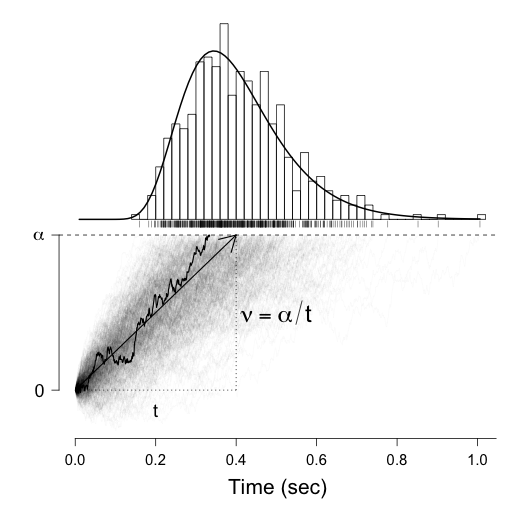
\includegraphics[width=\linewidth]{figures/wald_distribution.png}
    \caption{Illustration of the process that results in a Wald distribution. Evidence starts at 0 and accumulates as a Wiener process with a drift $\nu$ (displayed as arrow) until it reaches a threshold $\alpha$. The process is inherently noisy as shown by 500 different traces generated with the same parameters (grey lines). The first passage time (the time it takes to trespass the threshold $\alpha$ for the first time) results in a Wald distribution (displayed on top).}
    \label{fig:wald_distribution}
\end{figure}

Other models contain similar data generating processes. For example, ICAT \citep{trukenbrod2014icat} relies on the concept of autonomous timer, which is thought of as a stochastic discrete state that rises to a threshold. The difference between our proposal and ICAT (apart from the discreteness) is what the rise to threshold depends on --- as the name suggests, autonomous timer depends on internal processes, a "biological clock", whereas our accumulator depends not only on internal characteristics of the observer, but their surroundings as well.

\subsection{Model for \textit{where}}

After the observer concludes that there is an advantage to move to another location, it is time to make a saccade.

Each location of the stimulus provides some amount of attraction to the observer. We call a function that maps the stimulus coordinates to that attraction an \textit{intensity} function and denote it as: $\lambda: \mathbb{R}^2 \rightarrow \mathbb{R}_+$, and will write it as $\lambda(x, y | s)$, where $s$ stands for the current fixation. The total amount of intensity of the whole stimulus is the integral (sum) of all the points of the stimulus: $\Lambda = \int\int \lambda(x, y | s)~dx dy$. In essence, we assume that when observers decide \textit{where} to go next, they pick a random location from a distribution proportional to this function. The function may or may not depend on the current or previous fixations, depending on whether we assume a homogeneous (static over time) or heterogeneous (evolving over time) process, and can be adjusted depending on the researcher's questions and desires.

In general, we will represent the intensity function as combination of different factors that influence the intensity of different locations. These factors may represent different features and can be combined in different ways \citep[see][]{barthelme2013spatial}. For example, we can build the intensity function such that it combines bottom up features of the stimulus (e.g., saliency) with systematic tendencies (e.g., central bias or horizontal bias), and so forth. Some of the factors can be thought of as representing information provided by the stimulus, assuming that locations that are rich in the information they provide will be attractive to fixate --- and so will have a high intensity. However, people not always fixate on locations with a lot of information. Later, it will be important to make a distinction between two types of factors that combine in the intensity. The first group of factors will encompass those that in some sense represent, or encode, information provided by the stimulus, such as objects, shapes, colors, edges, faces, etc.\footnote{We use the term \textit{information} for a lack of a better word, and do not use it in a strict sense associated with the work of \citet{shannon1948communication}.} We will denote the combination of these factors as $\lambda_1(x, y |s)$ and the integral $\Lambda_1 = \int\int \lambda_1(x, y | s)~dx dy$ will represent the total amount of information provided by the stimulus. The second group comprises of factors that do not represent information of the stimulus but influence the attractiveness of the potential locations by another way, for example heightening the intensity near the center of the stimulus would represent a central bias.


\subsection{Combining models for \textit{when} and \textit{where}}

Human vision is limited by that the most detail available is at a particular part of the retina: fovea, a place where the light falls from roughly around the center of gaze. The physiological aspects of foveal, parafoveal and extrafoveal vision are out of the scope of this article, but similarly to the previous attempts for modeling of eye movements \citep{trukenbrod2014icat, schutt2017likelihood,schwetlick2020ccenewalk_extendeds}, we represent the fact that vision is sharpest inside the fovea by implementing a so called "attentional window". This window suppresses intensity of locations relatively farther from the center of gaze.


In essence, we define an attentional window as a function $a:~\mathbb{R}^2~\rightarrow~\mathbb{R}~\in~[0, 1]$ and denote it as $a(x, y | s)$, where $s$ stands for the $x$ and $y$ coordinates of the current fixation. The value of $a$ corresponds to the proportion of the intensity of locations at $(x, y)$ given the current fixation location $s$. To get a representation of the actual intensity of different locations, given a particular fixation location $s$, we can multiply the intensity function by this attentional window: $\omega(x, y | s) = a(x, y | s)\times\lambda(x, y | s)$, and the total amount of accessible intensity during a particular fixation $s$ is $\Omega = \int\int \omega(x, y | s)~dx dy$ (the total amount of information accessible to the observer at a particular location will be denoted as $\Omega_1 = \int\int \omega_1(x, y | s)~dx dy = \int\int a(x, y | s)\times\lambda_1(x, y | s)~dx dy$). Figure~\ref{fig:attention_window} illustrates this concept with examples in one dimension.

\begin{figure}
    \centering
    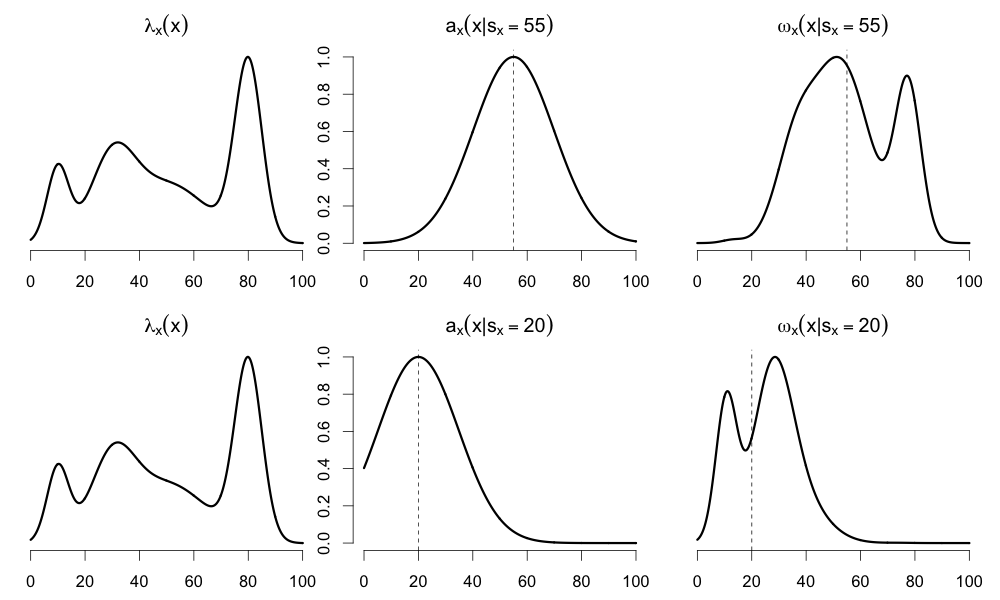
\includegraphics[width=\linewidth]{figures/attention_window.png}
    \caption{The left panel shows an example intensity function $\lambda(x)$ as a function of location along the $x$-coordinate. The middle panel shows the attention window given that the current fixation is at $s_x = 55$ (top) or $s_x=20$ (bottom). The right panel shows the intensity accessible through the attention window.}
    \label{fig:attention_window}
\end{figure}

The concept of attentional window is important in our model as it provides a link between the model for \textit{when} and model for \textit{where} to enable dependencies between the two. In the model for \text{when}, the time it takes the observer to make a decision (to make a saccade) can be modelled as a Wald distribution with parameters drift $\nu$ and decision boundary $\alpha$. However, it is likely that fixation durations vary depending on the surrounding of the current fixation locations \citep{nuthmann2010crisp,nuthmann2017fixation_durations}. 

The dependency of the fixation durations on fixation locations can be created in two ways. Both approaches rely on the distinction between factors that do and do not represent information provided by the stimulus, as we assume that only information has a potential to influence the fixation duration (e.g., fixating on a location particularly rich on detail will take longer on average than on a location with only a uniform background) and not other factors that do not provide information (e.g., central bias can attract people to make a saccade towards the center of the screen, but there is no immediately plausible mechanism for having longer fixation durations in the center of the screen compared to the edges just because it is in the center).

In the first approach, we can assume that upon arriving to a location $s$, the observer harvests information from around that location with a drift rate $\nu$, and once the information available from that location is depleted, the decision to \textit{Go} is activated. In this framework, the total amount of information available through the attention window $\Omega_1$ would replace the decision boundary $\alpha$ in the Wald model.

In the second approach, we can adopt the idea from LATEST \citep{tatler2017latest} that the decision to make a saccade is based on continual comparison of two hypotheses (\textit{Stay} vs \textit{Go}), where the "evidence" is based on the information provided if one or another decision is adopted. The evidence supporting the decision to stay is the total amount of information accessible through the attention window ($\Omega_1$), whereas the evidence supporting the decision to Go is the total amount of information provided by the stimulus ($\Lambda_1$). In this framework, the drift rate of the Wald model is replaced by the log of the ratio of the two evidences:

\begin{equation}
\nu = \ln\left(\frac{Go}{Stay}\right) = \ln\left(\frac{\Lambda_1}{\Omega_1}\right),
\end{equation}

and the evidence accumulation continues until the decision threshold $\alpha$ is reached.

\section{Concrete model}

In the previous section, we tried to describe the model in conceptual terms. However, in order to implement the model, there are several choices to be made in regards how to model the contribution of different factors, including their functional forms. Some of these choices will be purely pragmatic and statistical rather than theoretical, and are mostly motivated by the requirement to have a computationally tractable and modifiable model.

The model can be difficult to implement due to the two-dimensional integrals that are used to obtain the values of $\Lambda_1$ (total information on the stimulus) and $\Omega_1$ (total information available through the attention window). The analytic tractability of these integrals relies on the functional form of the functions $\lambda(x, y)$ and $a(x, y)$, and consequently $\omega(x, y)$. This obstacle can be solved in two ways. 

First, it is possible to divide the stimulus into a grid of discrete locations, leading to an approximation of the continuous space, which leads to tractability regardless of the functional forms (i.e., integrals become sums) at the expense of loosing precision due to the discrete approximation. The degree of precision is arbitrary as it can be increased or decreased by changing the size of the cells in the grid, but could quickly lead to a computational bottleneck for fine grained approximations due to the explosion of the number of terms to be summed.

Second, the construction of the functions at play can be carefully selected such that the integrals are analytically tractable. This severely limits the flexibility of the model as it does not allow for very many choices, but avoids the arbitrary choice of the precision to be used when using the discrete approximation approach.


\subsection{Modeling $\lambda$}

The model for the function $\lambda$ that converts the coordinates of the stimulus to intensity can be achieved in different ways. We generally desire to include different factors in the model, for example central and directional biases, information about locations of objects on the scene, etc. This can be achieved by following \citep{barthelme2013spatial}:

\begin{equation}
    \lambda(x, y) = \Phi \left(\sum \beta_k f_k(x, y) \right),
\end{equation}
where $\beta_k$ is a weight of a factor $k$, $f_k$ is a function that maps factor $k$ to the locations $(x, y)$, and $\Phi$ is analogous to a link function in GLMs. Particularly suitable candidates for this function are $\Phi (x) = \exp(x)$, $\Phi (x) = x$, $\Phi (x) = \ln(\exp(x) + 1)$ or their combinations \citep[see ][for the discussion of the differences between them]{barthelme2013spatial}. 

In our application, we use $\Phi$ to be an identity function, which by using appropriate restrictions (specified below Equation~\ref{eq:lambdaMixture}) results in a mixture model:

\begin{equation}
\label{eq:lambdaMixture}
    \lambda(x, y) = \sum \pi_k f_k(x, y),
\end{equation}
where $\pi_k \in [0, 1]$ and $\sum \pi_k = 1$, $f_k(x, y) \geq 0~\forall x, \forall y$, and $\int \int f_k(x, y) dx dy = 1$, making the $\lambda(x, y)$ a proper probability density over a plane. The value of $\pi_k$ then correspond to the relative importance of a factor $k$, and $f_k(x, y)$ corresponds to a distribution of $x$ and $y$ locations under that factor. By definition, the value of $\Lambda = 1$ (total intensity of stimulus) for whatever setting of the parameters. Particularly attractive property of such definition is the fact that the separation between the factors that represent information on the stimulus from the factors that do not is straightforward. For example, if the first and second factors ($k=1$ and $k=2$) encode objects on the screen and saliency (which can plausibly play a role in fixation durations), whereas the third factor ($k=3$) encodes a central bias (which arguably does not influence fixation durations) then simply $\lambda_1(x, y) = \pi_1 f_1(x, y) + \pi_2 f_2(x, y)$, and $\Lambda_1 = \pi_1 + \pi_2$.

Conceptually, such a formulation represents a generative model where the observer chooses the next fixation by first randomly selecting a factor $k$ with probability $\pi_k$ and then selects the location by randomly drawing from the density of the chosen factor $f_k$. It is questionable whether this assumption is the most realistic --- for example, taking $\Phi = \exp(x)$ (a log-additive model) correspond to observer combining all factors into one meshed weighted map which determines the next fixations, an approach taken by \citet{barthelme2013spatial}. We believe that which approach is more realistic can be partly addressed by empirical comparison of different models that differ in these kind of assumptions.


\subsection{Functional forms}

The crucial step is to determine the value of $\Omega$ (or $\Omega_1$) --- the total intensity available after filtering through the attention window $a(x, y |
s)$. Recall that: 

\begin{equation}
    \Omega = \int \int \omega(x, y) dx dy=  \int \int a(x, y) \lambda(x, y)dx dy.
\end{equation}

Given the specification of $\lambda$ introduced in Equation~\ref{eq:lambdaMixture}, we can rewrite it as:

\begin{equation}
\label{eq:GammaDoubleIntegral}
    \Omega = \int \int a(x, y) \sum \pi_k f_k(x, y) dx dy = \sum \pi_k \int \int a(x, y) f_k(x, y) dx dy,
\end{equation}
from which it is clearly visible that choice of the functional form of the attention window $a(x, y)$ and the individual factors $f_k(x, y)$ determine whether the model will be tractable without approximation through discretization. One of the possibilities to satisfy this is to model each $f_k(x, y)$ as a bivariate normal distribution, and $a(x, y)$ as a kernel of a bivariate normal distribution. Further, we will assume that the dimensions are uncorrelated, thus $f_k(x, y) = f_k(x)f_k(y)$ and $a(x, y) = a(x)a(y)$, where $f_k(.)$ is a Normal distribution with parameters $\mu_k$ and $\sigma_k$ for the appropriate dimensions, and $a(.)$ is similarly the gaussian kernel with center at the current fixation ($s$) and scale parameter $\sigma_a$ in the appropriate dimension. This allows us to rewrite the double integral in Equation~\ref{eq:GammaDoubleIntegral} into a product of two integrals:
\begin{equation}
    \Omega =  \sum \pi_k \int a(x)f_k(x) dx \int a(y)f_k(y) dy, 
\end{equation}
which has a simple analytic solution:
\begin{equation}
\begin{aligned}
\int a(x)f_k(x) dx = & \int \frac{1}{\sqrt{2\pi\sigma_k^2}} \exp\left[-\frac{(x-\mu_k)^2}{2\sigma_k^2}\right] \exp\left[-\frac{(x-s_x)^2}{2\sigma_a^2}\right]~dx = \\
= & \frac{1}{\sqrt{2\pi\sigma_k^2}} \int \exp\left[-\frac{(x-\mu_k)^2}{2\sigma_k^2} - \frac{(x-s_x)^2}{2\sigma_a^2}\right]~dx = \\
= & \frac{1}{\sqrt{2\pi\sigma_k^2}} \int \exp\left[-\frac{\sigma_a^2(x-\mu_k)^2 + \sigma_k^2(x-s_x)^2}{2\sigma_a^2\sigma_k^2} \right]~dx = \\
= & \frac{1}{\sqrt{2\pi\sigma_k^2}} \int \exp\left[-\frac{(\sigma_a^2+\sigma_k^2)\left(x-\frac{\sigma_a^2\mu_k + \sigma_k^2s_x}{\sigma_a^2+\sigma_k^2}\right)^2 + \frac{\sigma_a^2\sigma_k^2}{\sigma_a^2 + \sigma_k^2}(\mu_k-s_x)^2}{2\sigma_a^2\sigma_k^2} \right]~dx = \\
= & \frac{1}{\sqrt{2\pi\sigma_k^2}} \exp\left[-\frac{(\mu_k-s_x)^2}{2(\sigma_a^2 + \sigma_k^2)}\right] \int \exp\left[-\frac{(\sigma_a^2+\sigma_k^2)\left(x-\frac{\sigma_a^2\mu_k + \sigma_k^2s_x}{\sigma_a^2+\sigma_k^2}\right)^2}{2\sigma_a^2\sigma_k^2} \right]~dx = \\
= & \frac{1}{\sqrt{2\pi\sigma_k^2}} \exp\left[-\frac{(\mu_k-s_x)^2}{2(\sigma_a^2 + \sigma_k^2)}\right] \sqrt{2\pi} \sqrt{\frac{\sigma_a^2\sigma_k^2}{\sigma_a^2+\sigma_k^2}} = \\
= & \frac{\sigma_a}{\sqrt{\sigma_a^2+\sigma_k^2}} \exp\left[-\frac{(\mu_k-s_x)^2}{2(\sigma_a^2 + \sigma_k^2)}\right],
\end{aligned}
\end{equation}
and equivalently in the $y$ dimension.

Finally, we use the parametrization where the drift rate $\nu$ varies with the location of the fixation. Combining the previous two equations, we can write the drift rate as follows:

\begin{equation}
\label{eq:nuAsLogOmega}
\begin{aligned}
\nu | s, \sigma_a, \lambda & = \ln(\Lambda_1) - \ln(\Omega_1) = \ln(\Lambda_1) - \ln(\Omega_1) \\
& = \ln\sum_{k=1}^K \pi_k- \ln \sum_{k=1}^K \exp \Bigg[\ln \pi_k + \sum_{i=1}^2 \Big( \ln \sigma_{ai} - \frac{\ln (\sigma_{ai}^2+ \sigma_{ki}^2)}{2} - \frac{(\mu_{ki} - s_i)^2}{2(\sigma_{ai}^2 + \sigma_{ki}^2)} \Big)  \Bigg],
\end{aligned}
\end{equation}
where the iteration over $i$ only makes explicit the integration over $x$ and $y$ dimensions. The above expression was purposely written in the log-sum-exp-log form explicitly to bring it in line with its computational implementation (which is more stable in this form). In case not all factors provide information, the only change in Equation~\ref{eq:nuAsLogOmega} would be the term $K$ in the first summation (e.g., if the first two factors belong to $\lambda_1$ but not the third, $K=3$ would be replaced with $K=2$).

\subsection{Likelihood}


Assuming data in the form of $d \in \mathbb{R}_+^T$ as the durations and $s = (s_x, s_y) \in \mathbb{R}^{T\times2}$ as the $x$ and $y$ coordinates of $T$ observed fixations, the likelihood of the model can be written as:
\begin{equation}
    \mathcal{L}(\theta | d, s) = \prod_{t=1}^T \lambda^{(t)}(s_x^{(t)}, s_y^{(t)} | \pi, \mu, \sigma) \times f_{W}(d^{(t)} | \nu^{(t)}, \alpha),
\end{equation}
where the superscript for $\lambda$ means that the intensity function might change during the course of time (which we show later), and $\nu^{(t)}$ changes depending on the current location through Equation~\ref{eq:nuAsLogOmega}. $f_W$ stands for the p.d.f. of the Wald distribution.

In general, assuming $K$ factors included in the model, the model can have $K$ parameters $\pi_1, ..., \pi_K$, $2\times K$ parameters $\mu_1, ..., \mu_K$ (each a vector of 2 for $x$ and $y$ direction), $2\times K$ parameters $\sigma_1, ..., \sigma_K$ (each a vector of 2 for the $x$ and $y$ directions), 2 parameters for $\sigma_a$ (the width of the attention window in the $x$ and $y$ directions), and $\alpha$, totalling $5K + 3 - 1$ free parameters. Depending on the actual factors included in the model, we will be able to fix or equate some parameters to reduce the number of parameters to be estimated, although it is not necessary to do so.

% \section{Case Studies}

% The model described above is very general and can take a variety of specifications. Building a model to answer a specific question can thus take a bit of time and thought. 

% Here, we show how to build such a model from scratch, i.e., how to think about including different factors in the model. Specifically, in three steps, we will build a model that includes two systematic tendencies (central bias and direction bias), and one top-down factor (positions and sizes of objects on the screen).

% The purpose of this section is to initiate the reader into building a model based on our proposal, show that the model is able to recover parameters from simulations, and how to assess the adequacy of the model. The section is accompanied with an online supplemental material (url) that shows, step by step, the implementation of the model in a statistical modelling language Stan (Carpenter, et al., xxx). We believe that such an approach will help potential user of our model to change the model specification according to their research question and application, while holding oneself to the highest possible standards of robust cognitive modeling (Lee et al, 2019; Shad, Bentacour, \& Vasishth, 2019; Bentacour, 2018).




% \subsection{Central bias}

% Central bias is one of the empirically observed systematic tendencies that bias the distribution of fixations towards the center of the screen (Tatler, et al.). 

% We start with building the model including only central bias. Including only one factor in the model is very easy and unrealistic, but it allows to demonstrate the core basic of the model clearly.

% Given that we have only one factor, the summation over all factors in Equations~\ref{eq:lambdaMixture} and \ref{eq:nuAsLogOmega} drop out, as well as parameter $\pi$ which is by definition (Equation~\ref{eq:lambdaMixture}) equal to one. Further, by definition, central bias draws the fixations towards the center of the screen, and so the parameters in $\mu$ can be fixed to the coordinates of the center of the screen. 


% This leaves us with three parameters to estimate: $\alpha$ (the threshold in the Wald model), $\sigma_a$ (the width of the attention window), and $\sigma$ (the scale of the central bias). %We use weakly informative priors for these parameters: $\text{gamma}(\alpha = 2, \beta = 0.02)$ for $\sigma_a$ and $\sigma$, which draws the parameters a little bit away from zero, and places $91\%$ of the prior in the interval between 0 and 200 pixels, and has a long tail covering even larger values (the mode is about 50 and mean is 100). For $\alpha$, we use also weakly informative prior: Normal distribution truncated at 0 with mean parameter $1$ and standard deviation of 2.

% Due to the very simple nature of this model, many computations can be simplified and the resulting model can be written as follows:

% \begin{equation}
% \label{eq:CaseStudy_CentralBias}
% \begin{aligned}
%   s_x     & \sim \text{Normal}(\bar{x}, \sigma) \\
%   s_y     & \sim \text{Normal}(\bar{y}, \sigma) \\
%   d^{(t)} & \sim \text{Wald}(\nu^{(t)}, \alpha) \\
%   \nu^{(t)} & = - 2 \ln \sigma_a + \ln (\sigma_a^2 + \sigma^2) + \frac{\left(\bar{x} - s_x^{(t)}\right)^2 + \left(\bar{y} - s_y^{(t)}\right)^2}{2(\sigma_a^2 + \sigma^2)} \\
%   \sigma_a & \sim \text{Gamma}(., .) \\
%   \sigma   & \sim \text{Gamma}(., .) \\
%   \alpha   & \sim \text{Normal}(., .)_{[0, \infty]}
% \end{aligned}
% \end{equation}

% \subsection{Central bias + horizontal and vertical bias}


% \subsection{Central bias + horizontal and vertical bias + object oriented behavior}

\subsection{Including saliency}

An important branch of models that describe and predict distributions of fixation locations are saliency models. We define a classic saliency model as an algorithm that takes the image (stimulus) as an input, and which produces an output, usually by assigning each pixel a value representing the local saliency of that pixel. Common features that these models consider important are local-global contrasts in color, intensity, and edges.

Saliency models enjoy a lot of success in predicting eye movement behavior and thus it seems reasonable to include some form of a saliency map as one of the factors in our model. Unfortunately, given the nature of the output of saliency models, it is not possible to implement the model fully analytically, and we will instead resort to discretization.

Let's define a saliency map as $\mathbf{S}$, where each of its element assigns a saliency to a pixel. Having $I$ pixels in one dimension and $J$ pixels in the other dimension, we have a total number of $P = I \times J$ pixels. We can standardize the output of a saliency algorithm to ensure that $\sum_{p=1}^{P} \mathbf{s}_{p}~=~1$.

To include saliency into the model for \textit{where}, we obtain a representation of the saliency on a continuous space of the $x$ and $y$ coordinates by defining the intensity function of saliency as a two dimensional step function: 

\begin{equation}
\label{eq:saliency_where}
    f(x, y) = \frac{\mathbf{s}_{p(x,y)} }{h \times w},
\end{equation}
where $p(x, y)$ returns the index of a pixel which is a super set of the position $x$ and $y$, and where $h$ and $w$ is the height and width of the pixel. Standardization by the area of the pixel ensures that after converting the saliency map $\mathbf{S}$ to the intensity function, the volume $\int \int f(x, y)~dxdy$ amounts to 1.

To include saliency into the model for \textit{when}, we need to adopt additional simplifications as to evaluate the integral $\int \int a(x, y) \times f(x, y)~dxdy$. We define $x_p$ and $y_p$ as the $x$ and $y$ coordinates of the center of a pixel $p$, respectively, and approximate $f(x, y)$ as:

\begin{equation}
    f(x, y) \approx \sum_{p=1}^P \mathbf{s}_{p} \text{Normal}(x | x_p, \kappa)\text{Normal}(y | y_p, \kappa),
\end{equation}
which leads to (using results in Equation~\ref{eq:GammaDoubleIntegral}):

\begin{equation}
    \int \int a(x, y)f(x, y)~dx dy\approx \sum_{p=1}^P \mathbf{s}_{p} \frac{\sigma_a^2}{\sigma_a^2 + \kappa } \exp\left(-\frac{(x_p - s_x)^2+(y_p - s_y)^2}{2(\sigma_a^2 + \kappa)}\right),
\end{equation}
which we can further simplify by letting $\kappa \rightarrow 0$:

\begin{equation}
    \int \int a(x, y)f(x, y) \approx \sum_{p=1}^P \mathbf{s}_{p} \exp\left(-\frac{(x_p - s_x)^2+(y_p - s_y)^2}{2\sigma_a^2}\right).
\end{equation}

These steps enable us to approximately compute the drift rate by substituting the discrete saliency map with a continuous function.

However, this implementation still requires serious computational resources: for example, fitting a model that includes a saliency map of resolution of $800\times600$ pixels would mean summing up $P = 800\times600 = 480,000$ terms for every fixation in every iteration of the fitting procedure.

There are generally 3 ways to alleviate the problem of the computational complexity. First, it is possible not to include the discrete factor in the model for \textit{when}, but only include it into the factor for \textit{where}. However, leaving it out does not solve the problem, but rather avoids it altogether. Second, it is possible to downsample the output of the saliency map. Indeed, many saliency algorithms already output the saliency map that has a resolution smaller than the original image \citep[e.g., by a factor of $16$ in each of the dimensions,][] {itti1998model}. Having an input image of dimensions of $800\times600$ pixels then leads to quite substantial reduction: Instead of summing up 480,000 terms we need to sum up only about 2,000. Downsampling the saliency maps to have smaller resolution than the input image is also desirable from a measurement perspective as the eye-tracking devices likely have measurement error that translate to several pixels of the input image.  Downsampled saliency maps then correspond better to the level of precision of the data. Third, it is possible to limit the summation only for the terms that lie in a relative proximity from the current fixation. For example, the attention window lets through only at most $1.1\%$ of the total weights of the pixels that lie at a distance of $3\sigma_a$ or more, essentially meaning that many of the terms in the sum are basically zero. Leaving out the pixels that are that far from the current fixation can reduce the number of terms to be summed by a great amount while not sacrificing much of the computational accuracy. Downsampling and limiting the summations are not mutually exclusive and can be used at the same time --- an approach we take in the practical implementation of our model.



\section{Application}

Here, we apply a particular realization of the model to data by \citet{renswoude2019object_familiarity} to demonstrate its use in applied context.

In this application, we are interested in the extend to which four different factors influence the distribution of fixation locations and the timing of saccades. 

The four factors that we considered are the 1) locations (and sizes) of objects on the scene \citep{xu2014beyond,renswoude2019object_familiarity}, 2) saliency \citep{itti1998model,itti2000saliency,itti2001computational}, 3) exploitation \citep[i.e., tendency to make repeated fixations in a relative proximity to previous fixation;][]{malem2020exploration}, and 4) central bias \citep{renswoude2019central}. 

As an inherent product of the model, we will also obtain assessment of the individual differences between the participants in terms of their tendency to dwell longer on current locations (captured by the decision boundary), and the width of their attention window.

\subsection{Data Descriptives}

The data contains recordings of 47 participants looking at 29 static pictures selected from the pool of 700 images created by \citet{xu2014beyond}. 39 participants looked at all 29 stimuli (min = 5, mean = 27.6, median = 29, max = 29 viewed images per participant). The mean number of fixations per trial was 11.4 (sd = 4.3); the total number of fixations in the data set is 14,807.

We split the data set in two parts, one of which we used to estimate the parameters of a model (number of fixations = 7,207), and one of which we used to validate the predictions of the model. We counter balanced the number of trials per participant in the two sets to ensure that both data sets contain some data from all participants and all items. The details of the procedure are available at \url{https://github.com/Kucharssim/DMEM/blob/master/scripts/prepare\_data.md}. 

\subsection{Initial Model}

The model contains four factors that determine the fixation locations, two of which are included in the model for fixation duration.

The model for where is composed of four factors, and so we can describe the distribution of fixation locations as follows:

\begin{equation}
    (x, y) \sim \sum_{k=1}^4 \pi_k f_k(x, y | \theta_k),
\end{equation}
where $\pi_k$ are the weights of different factors and $f_k$ is the distribution of a factor $k$ with parameters $\theta_k$.

The first factor is the location and sizes of objects on the scene. We assume that each object on the scene can have different level of attractivity and that larger objects distribute their total attractivity over larger area. This idea can be expressed by another mixture:

\begin{equation}
    f_1(x, y | \theta_1) = \sum_j \omega_j \text{Normal}(x | \text{center}_{xj}, \gamma \times \text{width}_{j}) \text{Normal}(y | \text{center}_{yj}, \gamma \times\text{height}_{j}), 
\end{equation}
where $\omega_j$ are the individual attractivities of different objects on a particular image, and that $\gamma$ is a scaling factor that stretches or compresses the attractivity of objects proportionally to their sizes.

The second factor is the saliency, which we treated as described in Equation~\ref{eq:saliency_where}.

The third factor can be described as an exploitation factor, and captures the phenomenon that people tend to linger close to the current fixation location: we model it as a bi variate normal distribution centered at the fixation location at time $t$ to predict the fixation location at time $t+1$:

\begin{equation}
    f_3(x, y|\theta_3) = \text{Normal}(x | s_x^t, \sigma_e) \text{Normal}(y | s_y^t, \sigma_e)
\end{equation}

The fourth factor represents the central bias, and is modelled as a bi variate normal distribution centered at the center of the screen ($x_c = 400$, $y_c = 300$)

\begin{equation}
    f_4(x, y|\theta_4) = \text{Normal}(x | 400, \sigma_d) \text{Normal}(y | 300, \sigma_d)
\end{equation}

For the fixation durations, we only consider the first two factors influential: the latter two factors do not stand for \textit{information} presented on the screen, but rather spatial biases, and therefore should not have any influence on saccade timing.

The model for fixation duration can be summarised as following.
\begin{gather*}
    d \sim \text{Wald}(\nu, \alpha) \\
    \nu = \ln(\pi_1 + \pi_2) - \ln\left(\int\int a(x, y | \sigma_a) \left(\pi_1 f_1(x, y | \theta_1) + \pi_2 f_2(x, y | \theta_2)\right)dxdy\right)
\end{gather*}

We implemented the model using the probabilistic programming language Stan \citep{carpenter2017stan} interfacing with R \citep{citeR} using the package \texttt{rstan} \citep{team2020rstan}.

\subsection{Results - Initial model}

We ran 10 MCMC chains with random starting values and default tuning parameters set by Stan. Each chain ran for 1,000 warm up and 1,000 sampling iterations, resulting in a total of 10,000 samples used for inference.
The model ran without any divergent transitions. We examined the potential scale reduction factor $\hat{\text{R}}$, trace plots, auto correlations, and the number of effective samples to identify potential problems with convergence. We did not find indications of poor convergence, and thus proceed with interpreting the model.


\textit{Posterior predictive checks.} We generated posterior predictives for the data set used for estimating the parameters to assess whether the fitted model reproduces the observed patterns in the data.

The model is able to capture the characteristic distribution of the fixation durations, as documented in Figure~\ref{fig:predictives_in_sample_durations}, although the model predicts a slightly fatter right tail than that of the data.

\begin{figure}
    \centering
    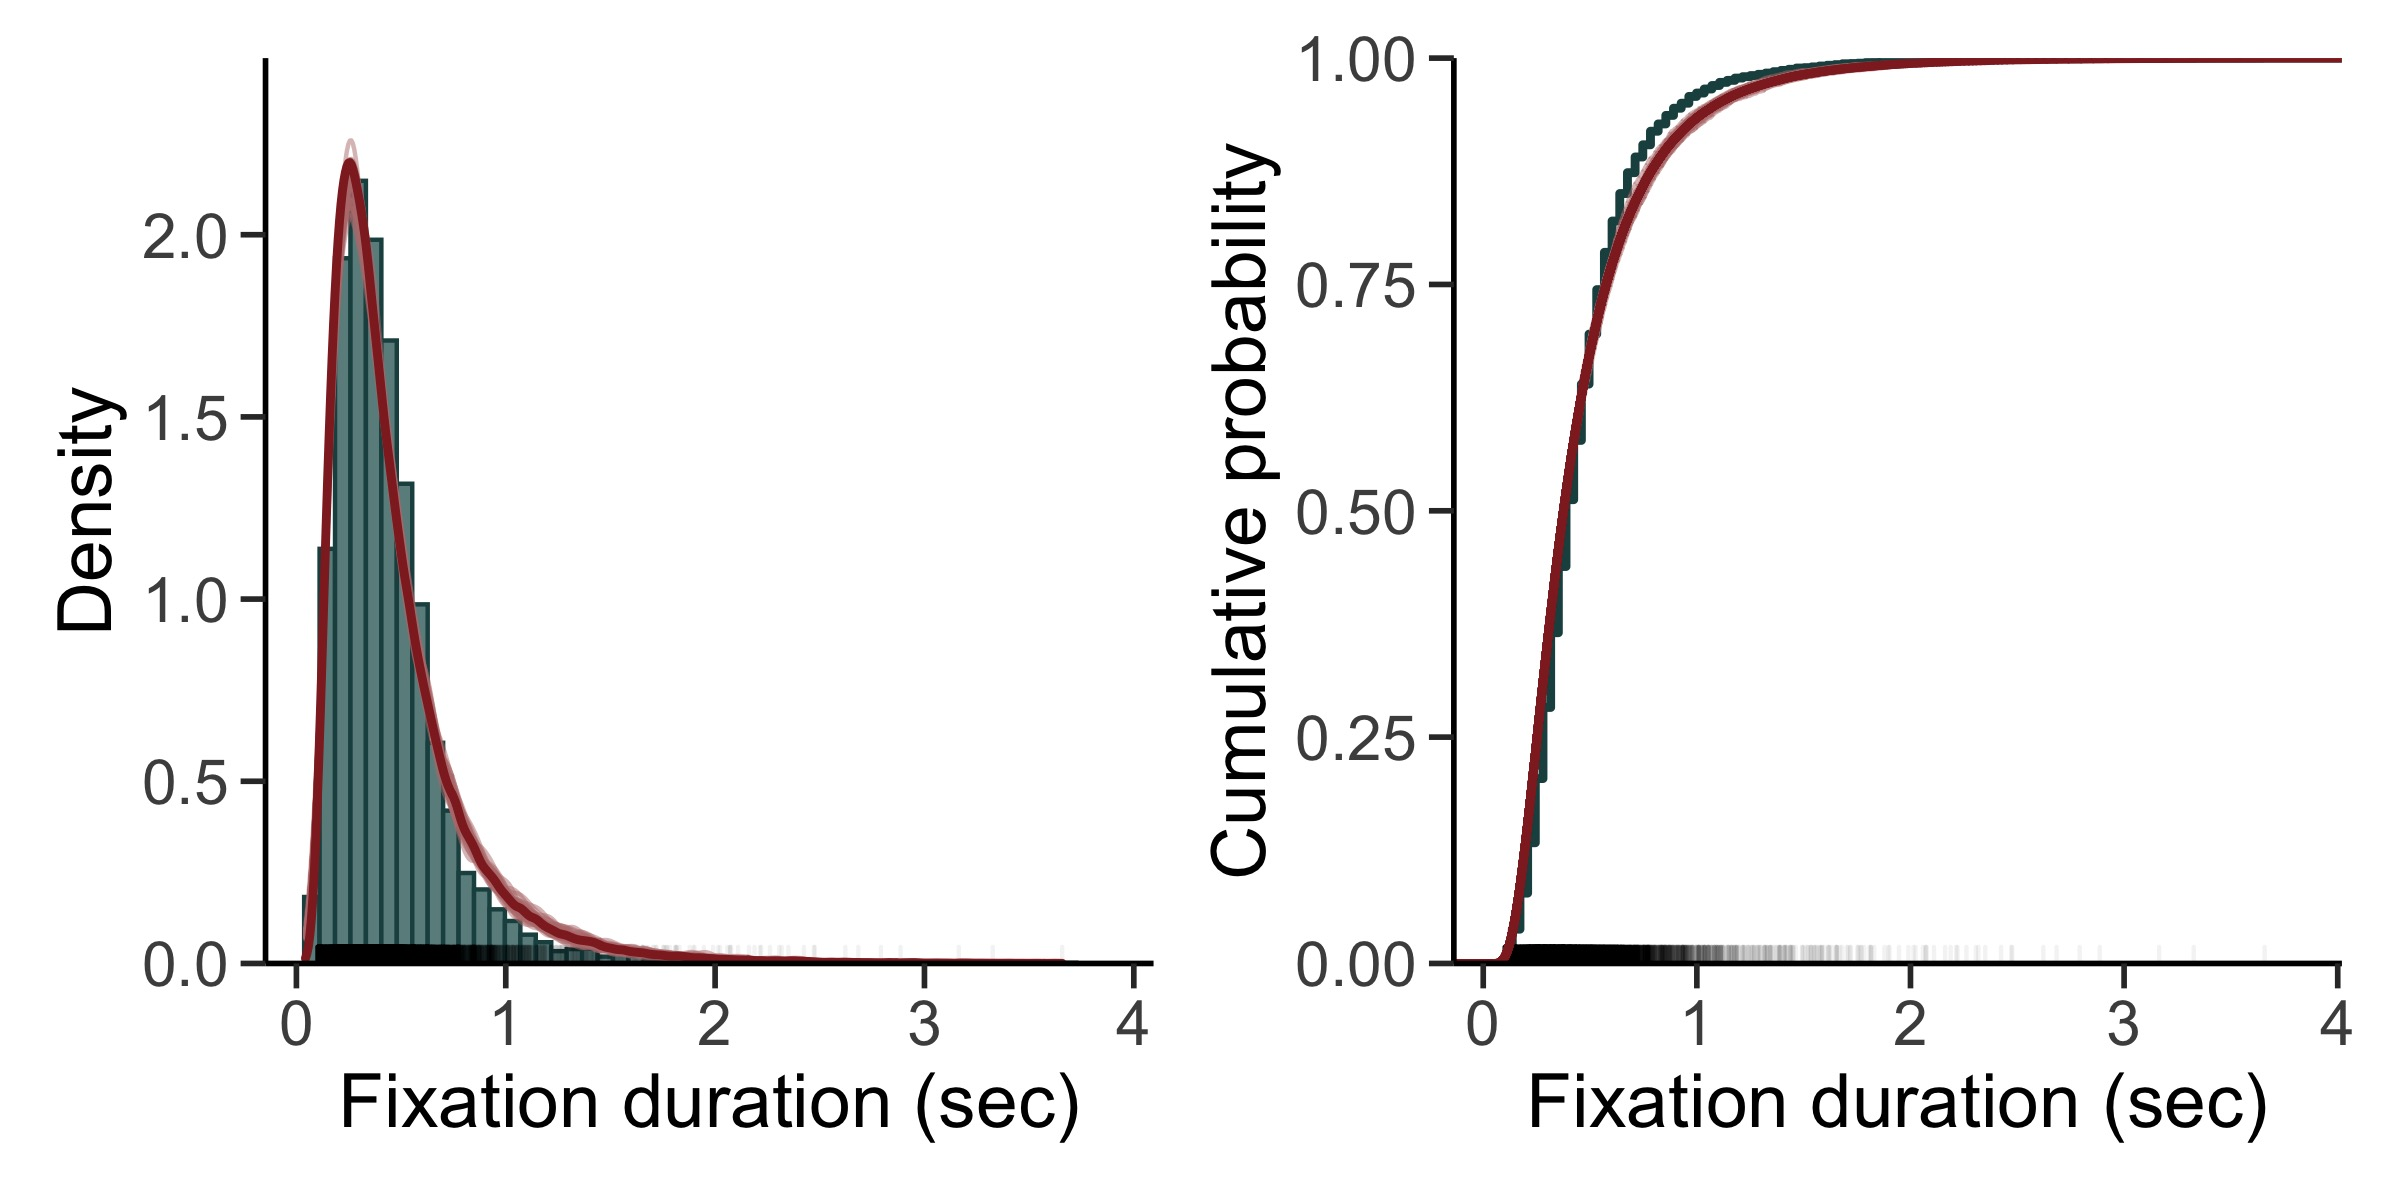
\includegraphics[width=\textwidth]{figures/fit_model/in_sample/fixation_durations.jpg}
    \caption{Predicted (red) versus observed (green) distribution of the fixation durations. Left panel shows histogram of the empirical data versus the density estimate using gaussian kernel of the posterior predictives. Right panel shows empirical cumulative distribution functions.}
    \label{fig:predictives_in_sample_durations}
\end{figure}

The model also reproduces the distributions of fixation locations.  Figure~\ref{fig:predictives_in_sample_xy} shows an example for one particular stimulus \citep[image number $251$ from][]{xu2014beyond}. The top-right in Figure~\ref{fig:predictives_in_sample_xy} displays the four factors included in the model, which combine proportionally to their weights to the posterior predictive distribution (labeled as predicted fixations).

\begin{figure}
    \centering
    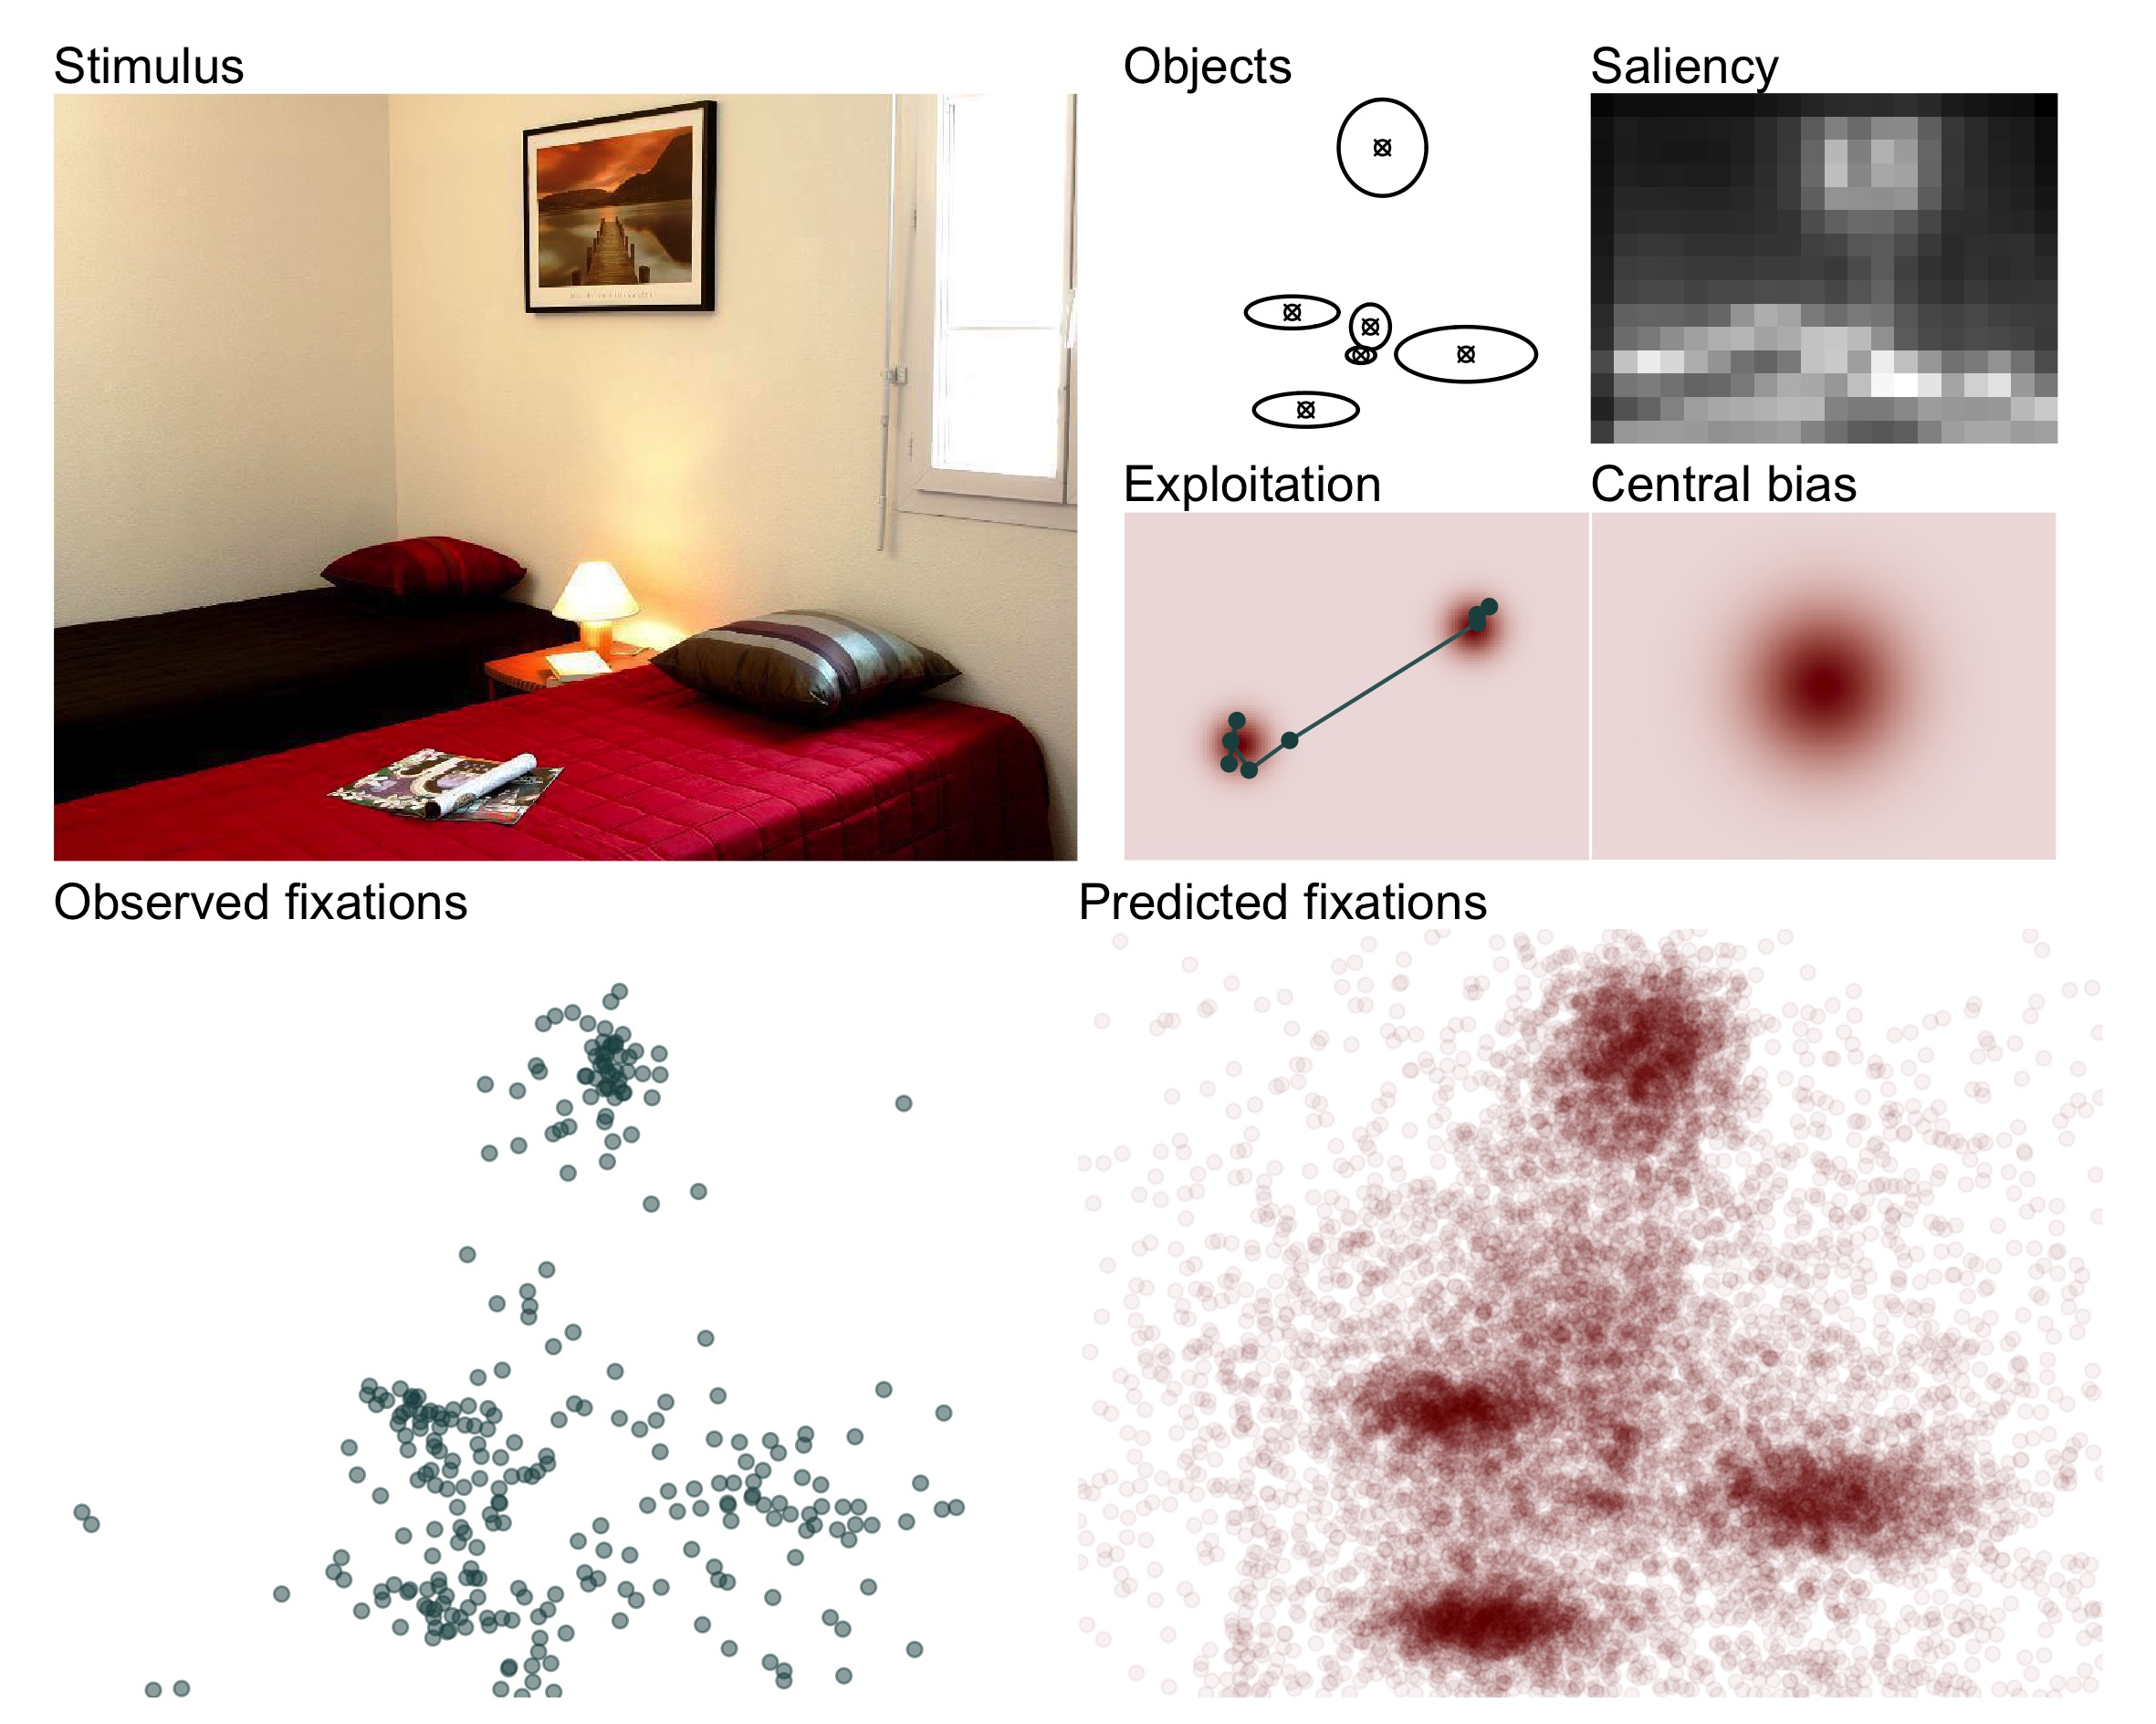
\includegraphics[width=\textwidth]{figures/fit_model/in_sample/xy/1251.jpg}
    \caption{Example of the model for fixation locations on the stimulus created by \citet{xu2014beyond} (top left panel). The four factors influencing the fixation locations are depicted in the top right quadrant. The bottom left panel shows the observed fixation locations, and the bottom right the draws from the posterior predictive distribution of the fitted model.}
    \label{fig:predictives_in_sample_xy}
\end{figure}

Next to the variables used to fit the data (fixation durations and fixation locations), we also checked at other quantities implied by the model. Specifically, we checked whether we can reproduce the distribution of saccade amplitudes and the distribution of saccade angles.  Saccade amplitude was measured as the Euclidean distance between two successive fixations in units of pixels. Saccade angle was calculated as an angle in radians between the horizontal axis of the screen and the vector that connects two successive fixations.

Figure~\ref{fig:predictives_in_sample_amplitude} shows the observed versus predicted distributions of saccade amplitudes on one example stimulus (shown in Figure~\ref{fig:predictives_in_sample_xy}). The model usually captures the distribution of saccade amplitudes relatively well, exhibiting two modes. Figure~\ref{fig:predictives_in_sample_amplitude} shows the observed versus predicted distributions of saccade amplitudes on the same stimulus. The prediction of saccade angles is relatively good on single stimuli, as usually the model predicts similar patterns of saccade directions (for example, Figure~\ref{fig:predictives_in_sample_angle} shows that the model captures saccade directions in the top-right and bottom-left directions). However, overall the model does not capture well an excess of saccades in the horizontal direction, which could be an indication that the model needs to be expanded with a factor that represents a horizontal bias \citep{renswoude2016horizontal}.

\begin{figure}
    \centering
    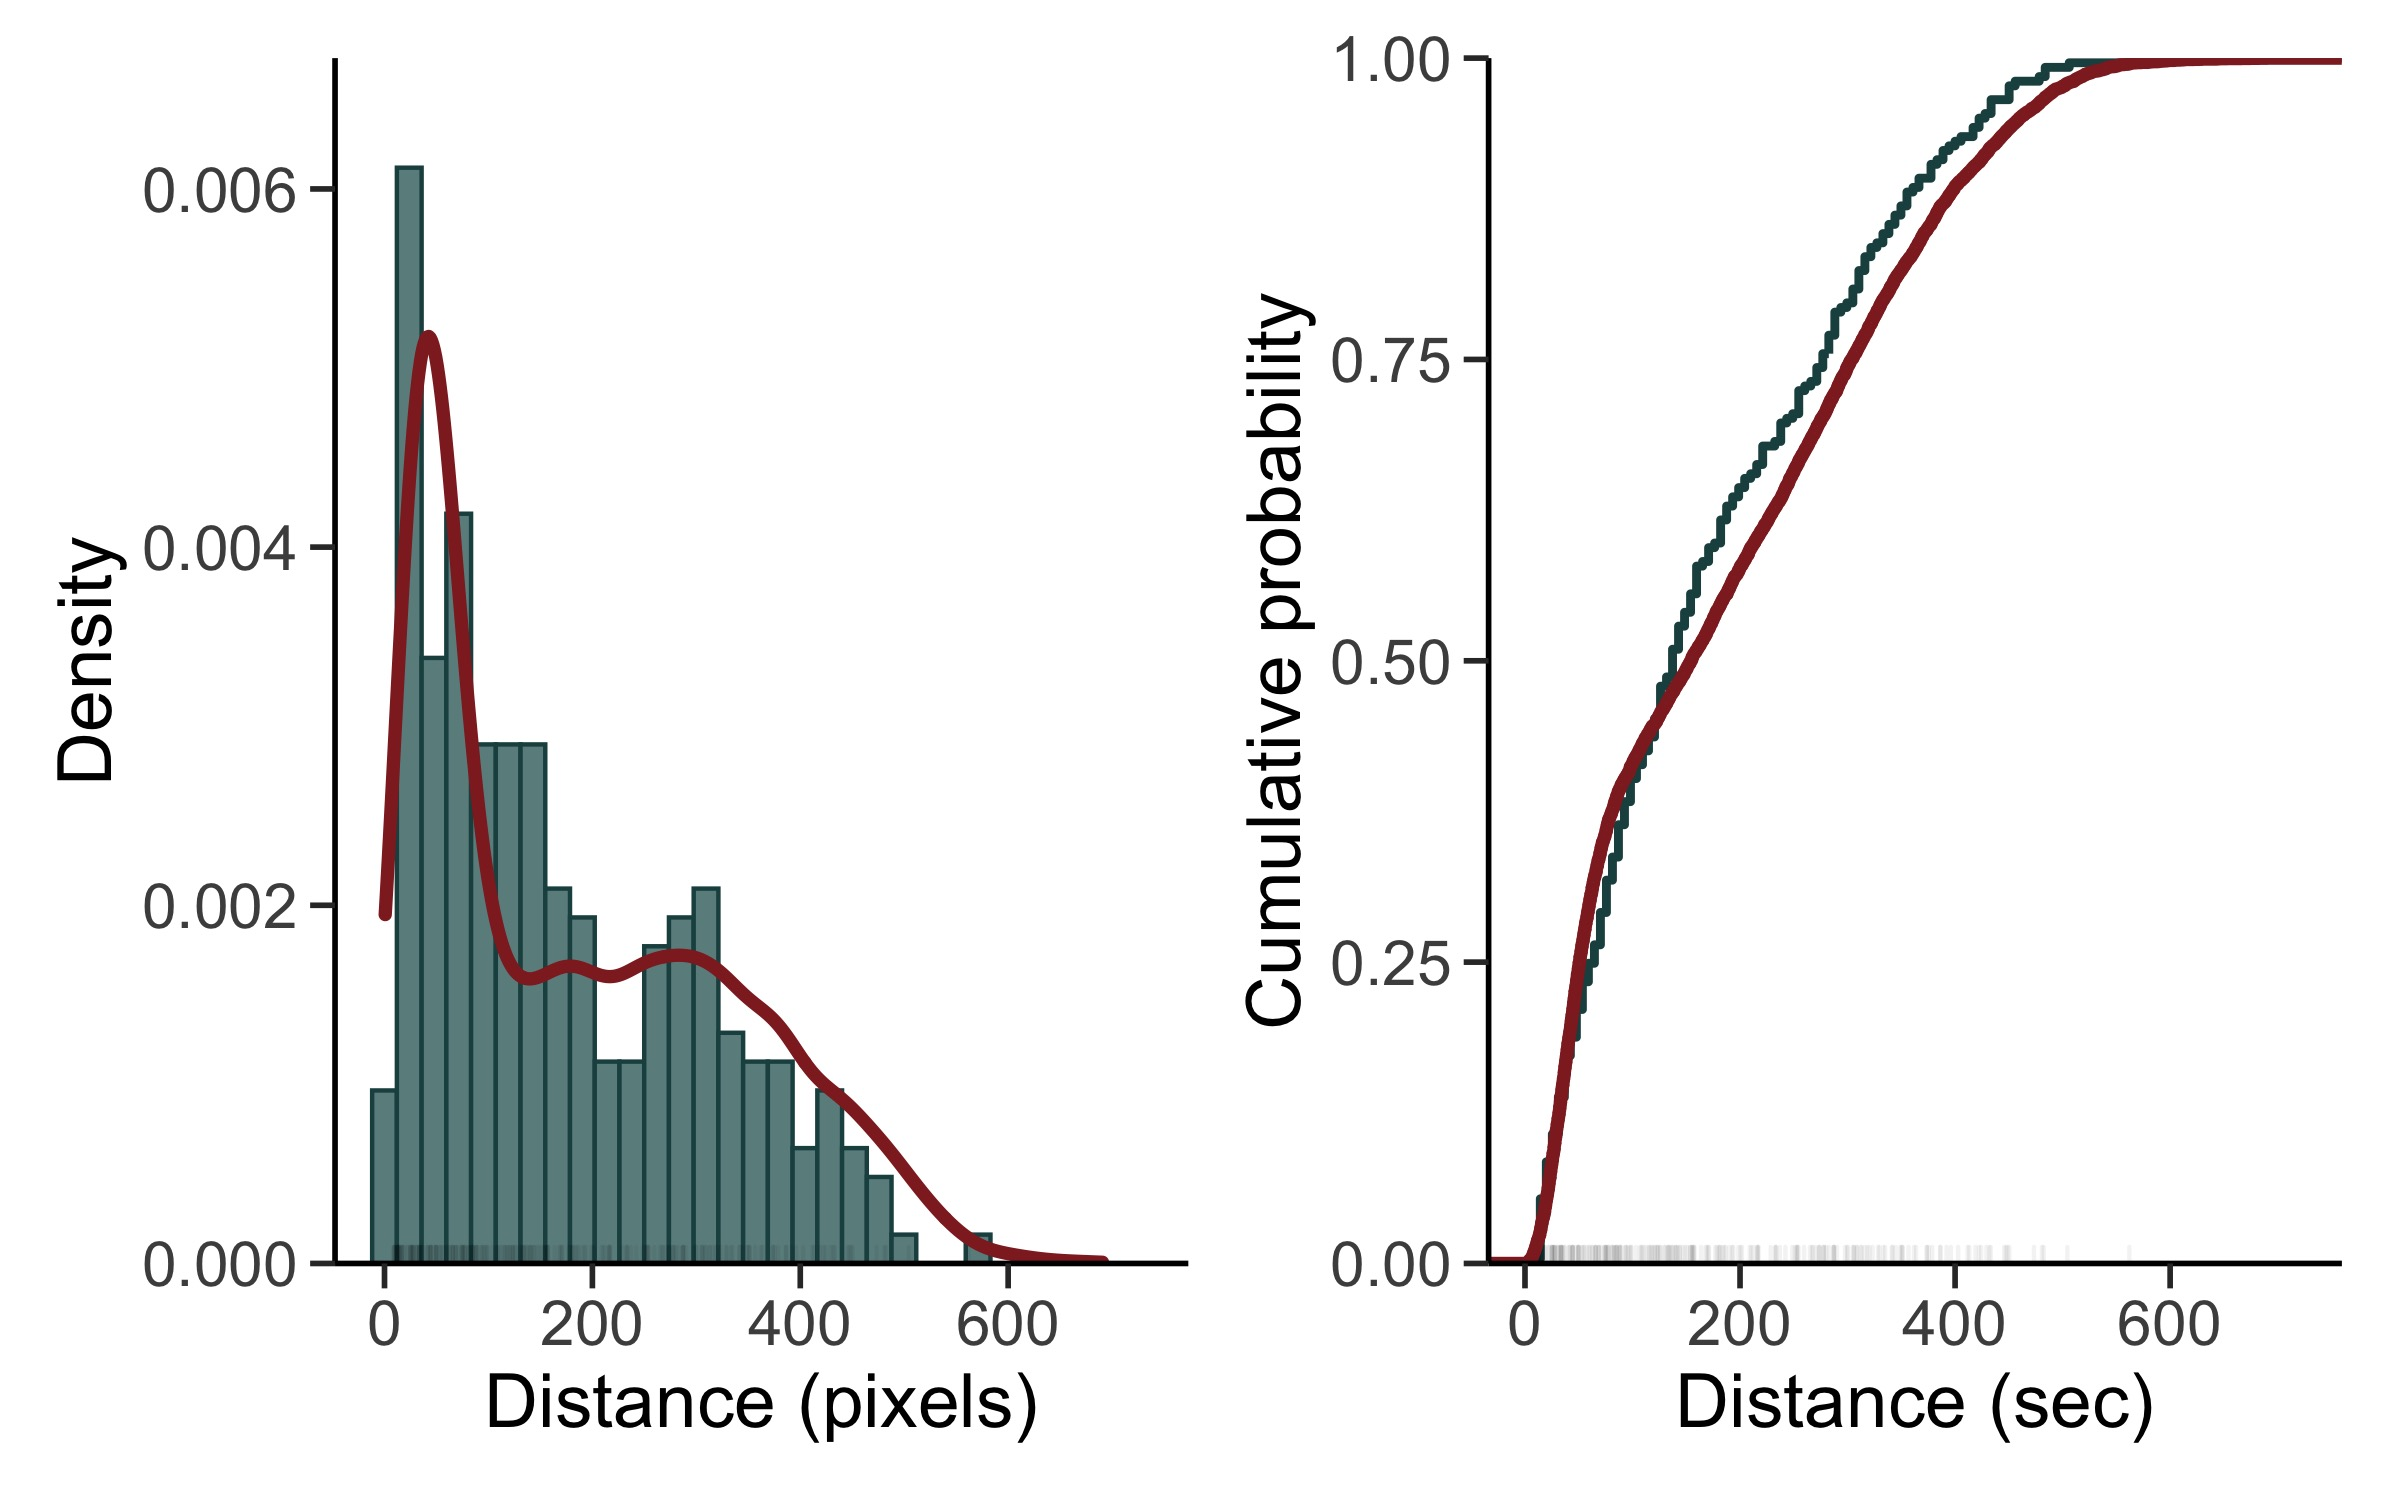
\includegraphics[width=\textwidth]{figures/fit_model/in_sample/amplitude/1251.jpg}
    \caption{Observed (blue) versus predicted (red) saccade amplitude on one particular stimulus (see Figure~\ref{fig:predictives_in_sample_xy}).}
    \label{fig:predictives_in_sample_amplitude}
\end{figure}

\begin{figure}
    \centering
    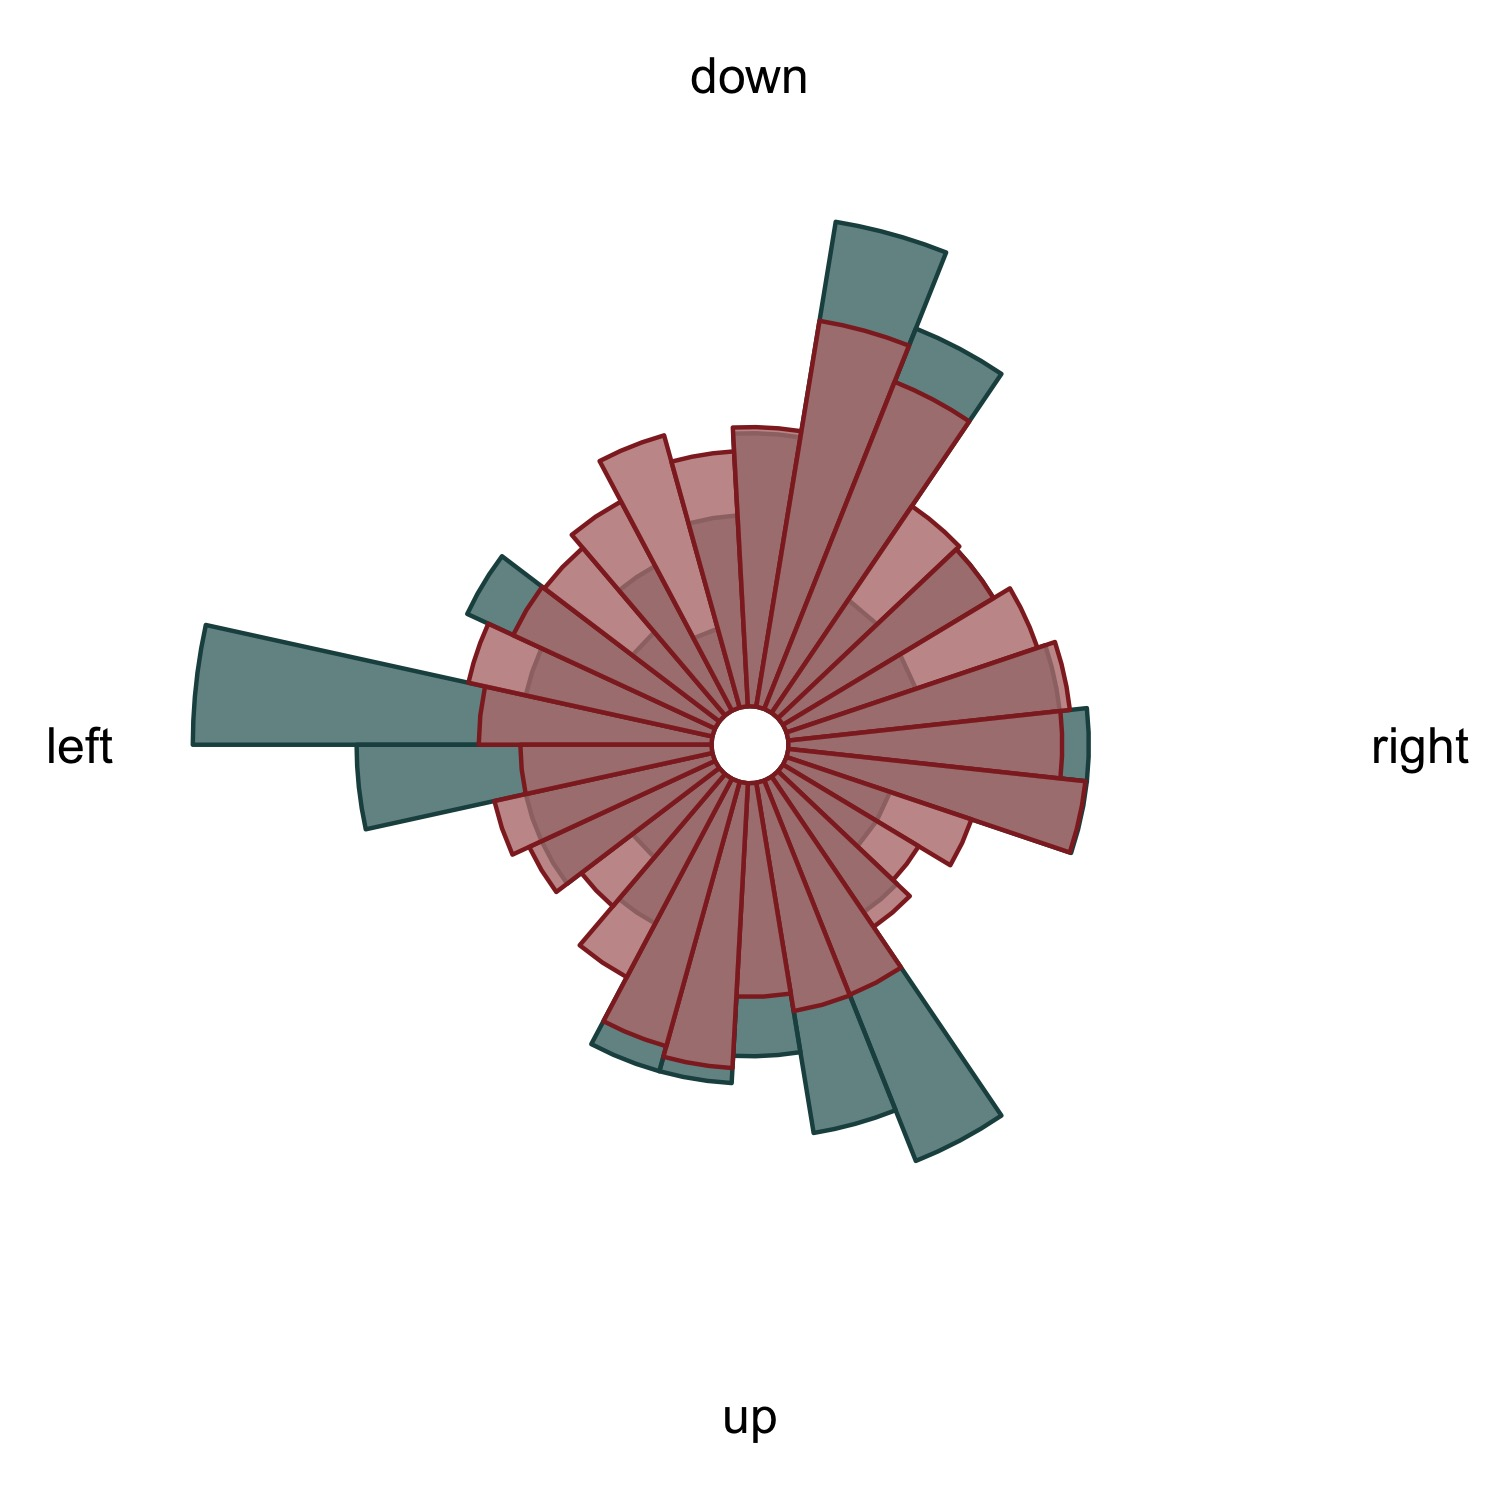
\includegraphics[width=0.4\textwidth]{figures/fit_model/in_sample/angle/1251.jpg}
    \caption{Observed (blue) versus predicted (red) saccade angle on one particular stimulus (see Figure~\ref{fig:predictives_in_sample_xy})}
    \label{fig:predictives_in_sample_angle}
\end{figure}

\textit{Parameter estimates}
The results indicated that the most important factor driving fixations was the locations of objects on the scene (weight = $0.37$, $95\%$ CI[$0.35$, $0.40$], followed by exploitation (weight = $0.30$, $95\%$ CI[$0.28$, $0.31$]), saliency (weight = $0.18$, $95\%$ CI[$0.16$, $0.20$]), and central bias (weight = $0.16$, $95\%$ CI[$0.14$, $0.17$]).

The parameter that controls sizes of objects as identified by \citet{xu2014beyond} indicated that people fixate relatively close to the centroids of the objects (scale = $0.23$, $95\%$ CI[$0.22$, $0.24$]). The exploitation region had a standard deviation $\sigma = 34.58$ ($95\%$ CI[$33.15$, $36.06$]) pixels, whereas the central bias region had a standard deviation $\sigma = 93.84$ ($95\%$ CI[$88.65$, $98.91$]) pixels.

\subsection{Extended model}

The original model fared well capturing the distribution of fixation durations and the overall distribution of fixation locations, and was able to a small degree capture an excess of horizontal saccades without this being explicitly built into the model. However the discrepancy between the model's predictions and data shown that the tendency to make horizontal saccades is particularly noteworthy and possibly needs an extra explanation.

To explore whether we can improve the model's capability to reproduce the amount of saccades in the horizontal direction, we extended the model. Specifically, we added another factor into the model for fixation locations, representing the horizontal bias. To create a factor that represents a saccadic bias (such as horizontal bias), instead of location preferences, it is possible to transform fixation locations (x and y coordinates) into a saccade representation (angle $\theta$ and amplitude $r$ of a saccade):
\begin{equation}
    \begin{aligned}
      \theta & = \text{arctan}\left(\frac{\Delta y}{\Delta x}\right) \\
      r & = \sqrt{\Delta x^2 + \Delta y^2},
    \end{aligned}
\end{equation}
where $\Delta x = x^t - x^{t-1}$ and $\Delta y = y^t - y^{t-1}$ represent a fixation as the difference of the x and y coordinates compared to the previous fixations (we set $x^0 = 400$ and $y^0 = 300$ as that is the middle of the screen).

That way, we can substitute a factor of locations with a factor of saccade angles and amplitudes:

\begin{equation}
    f(x, y) = \frac{f(\theta, r)}{r},
\end{equation}
where the denominator $r$ is the Jacobian determinant representing the stretching of the space after the change of variables from cartesian to polar coordinates: $dx dy = r dr d\theta$. 

To create the joint density of the angle and amplitude, we express it using the chain rule of probability:

\begin{equation}
    f(\theta, r) = f(\theta) \times f(r | \theta).
\end{equation}

The important part of this factor is the distribution of saccade angles, for which we specify the following distribution:

\begin{equation}
    f(\theta) = 0.5 \text{vonMises}(0, \kappa) + 0.5 \text{vonMises}(\pi, \kappa),
\end{equation}

which specifies a mixture of von Mises distributions with centers fixed to 0 and $\pi$ (i.e., right and left direction, respectively), and a concentration $\kappa$ which is estimated from the data. The mixture weights are fixed to $0.5$ as we assume that saccades in the left direction are equally attractive as saccades to the right direction.

The conditional density $f(r | \theta)$ is chosen to be a uniform stretched over the interval between 0 and the maximum saccade lenght that would not fall outside of the screen if it was launched from the position $(x^{t-1}, y^{t-1})$ under the direction $\theta$.

The generative mechanism for such a joint density is the following. First, observed draws a saccade angle from the distribution $f(\theta)$. Then, the observer draws a point along a line under the sampled angle $\theta$, that goes between location $(x^{t-1}, y^{t-1})$ and the edge of the screen. This point is the new fixation position.

Figure~\ref{fig:horizontal_example} shows and example of the function $f(\theta, r)$ on the screen coordinates, with $(x^{t-1}, y^{t-1})$ set to the center to the screen, and $\kappa = 15$.

\begin{figure}
    \centering
    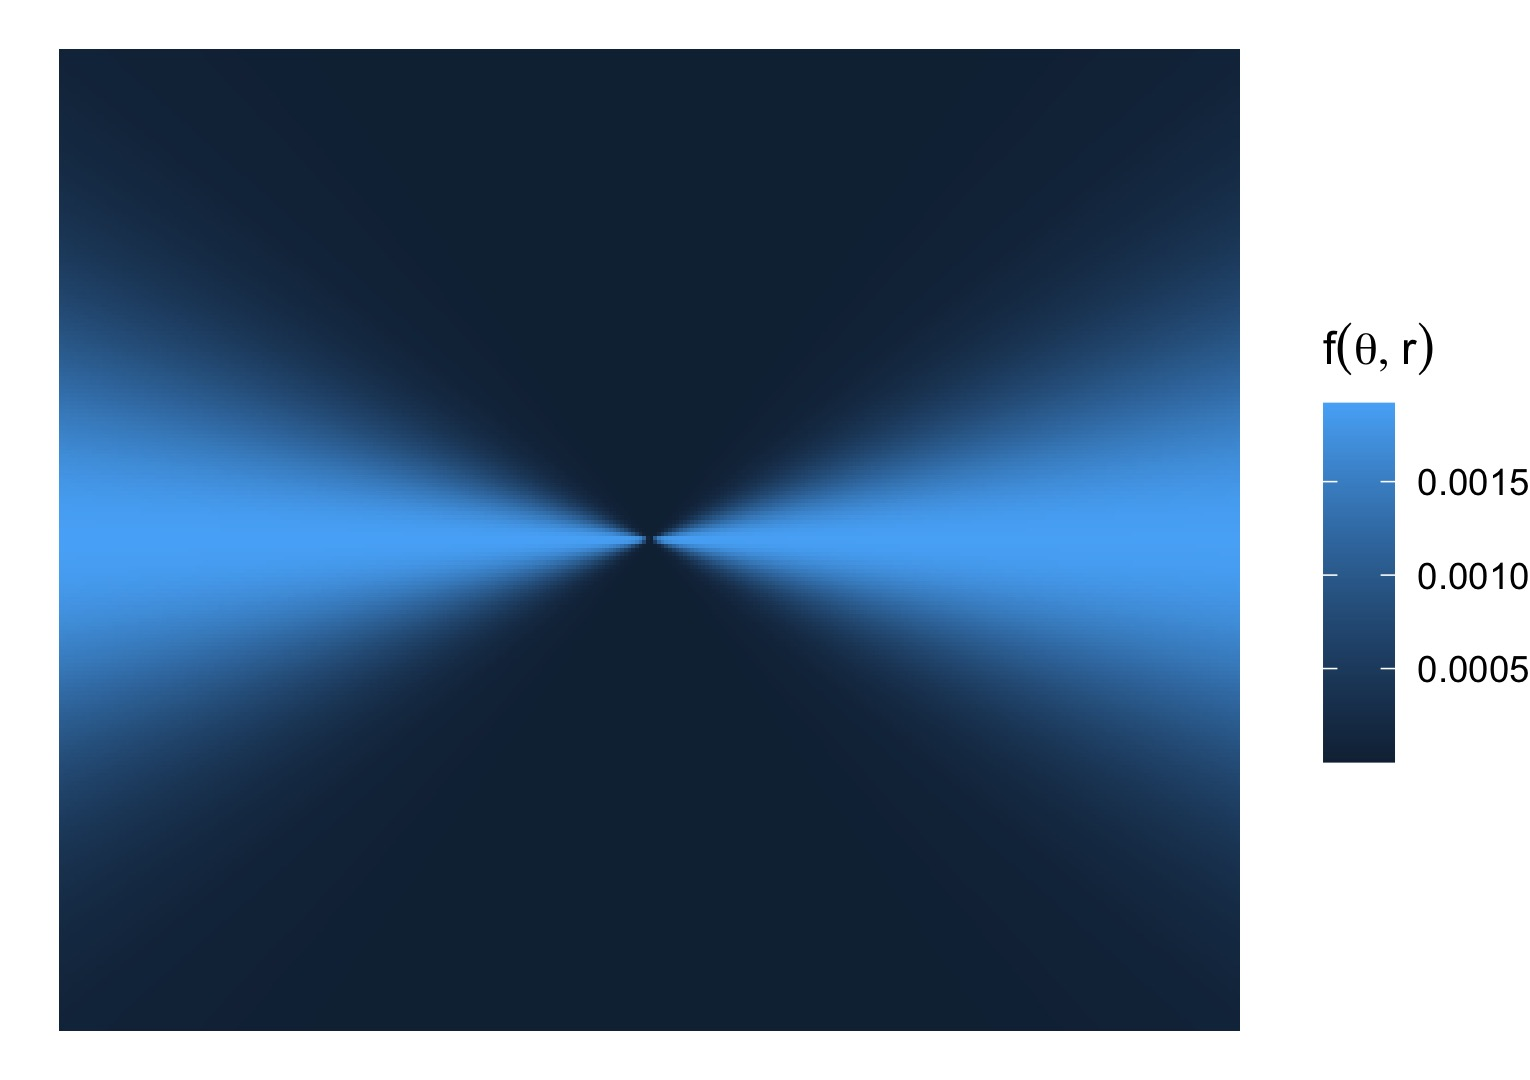
\includegraphics[width=\linewidth]{figures/horizontal_example.jpg}
    \caption{Example of the joint density of saccade angle and saccade amplitude plotted on the screen dimensions. The density highlights saccades in the left and right directions relative to the current fixation (in this figure, the center of the screen), representing the horizontal bias.}
    \label{fig:horizontal_example}
\end{figure}

The rest of the model stayed the same.

\subsection{Results - Extended model}

We fitted the extended model in the same way as the initial model: We run 10 MCMC chains with random starting values and default tuning parameters set by Stan. Each chain run for 1,000 warm up and 1,000 sampling iterations, resulting in a total of 10,000 samples used for inference. The model run withouth any divergent transitions. We examined the convergence diagnostics, to find that we could not identify potential problems with convergence. Thus, we proceed with interpreting the model.

\textit{Posterior predictive checks.} We conducted posterior predictive checks the same way as with the previous model: Comparing the predicted and observed distribution of fixation durations, fixation locations, saccade amplitudes, and saccade angles. The extended model performed similarly to the initial model in terms of the first three variables. As Figure~\ref{fig:horizontal_comparison} demonstrates, the extended model did better in terms of reproducing the overall distribution of saccade angles - being able to reproduce the excess of saccades going in the horizontal direction better after we have explicitly added a factor that represents horizontal bias. However, it is still visible that there is still some potential to improve the model predictions.

\begin{figure}
    \centering
    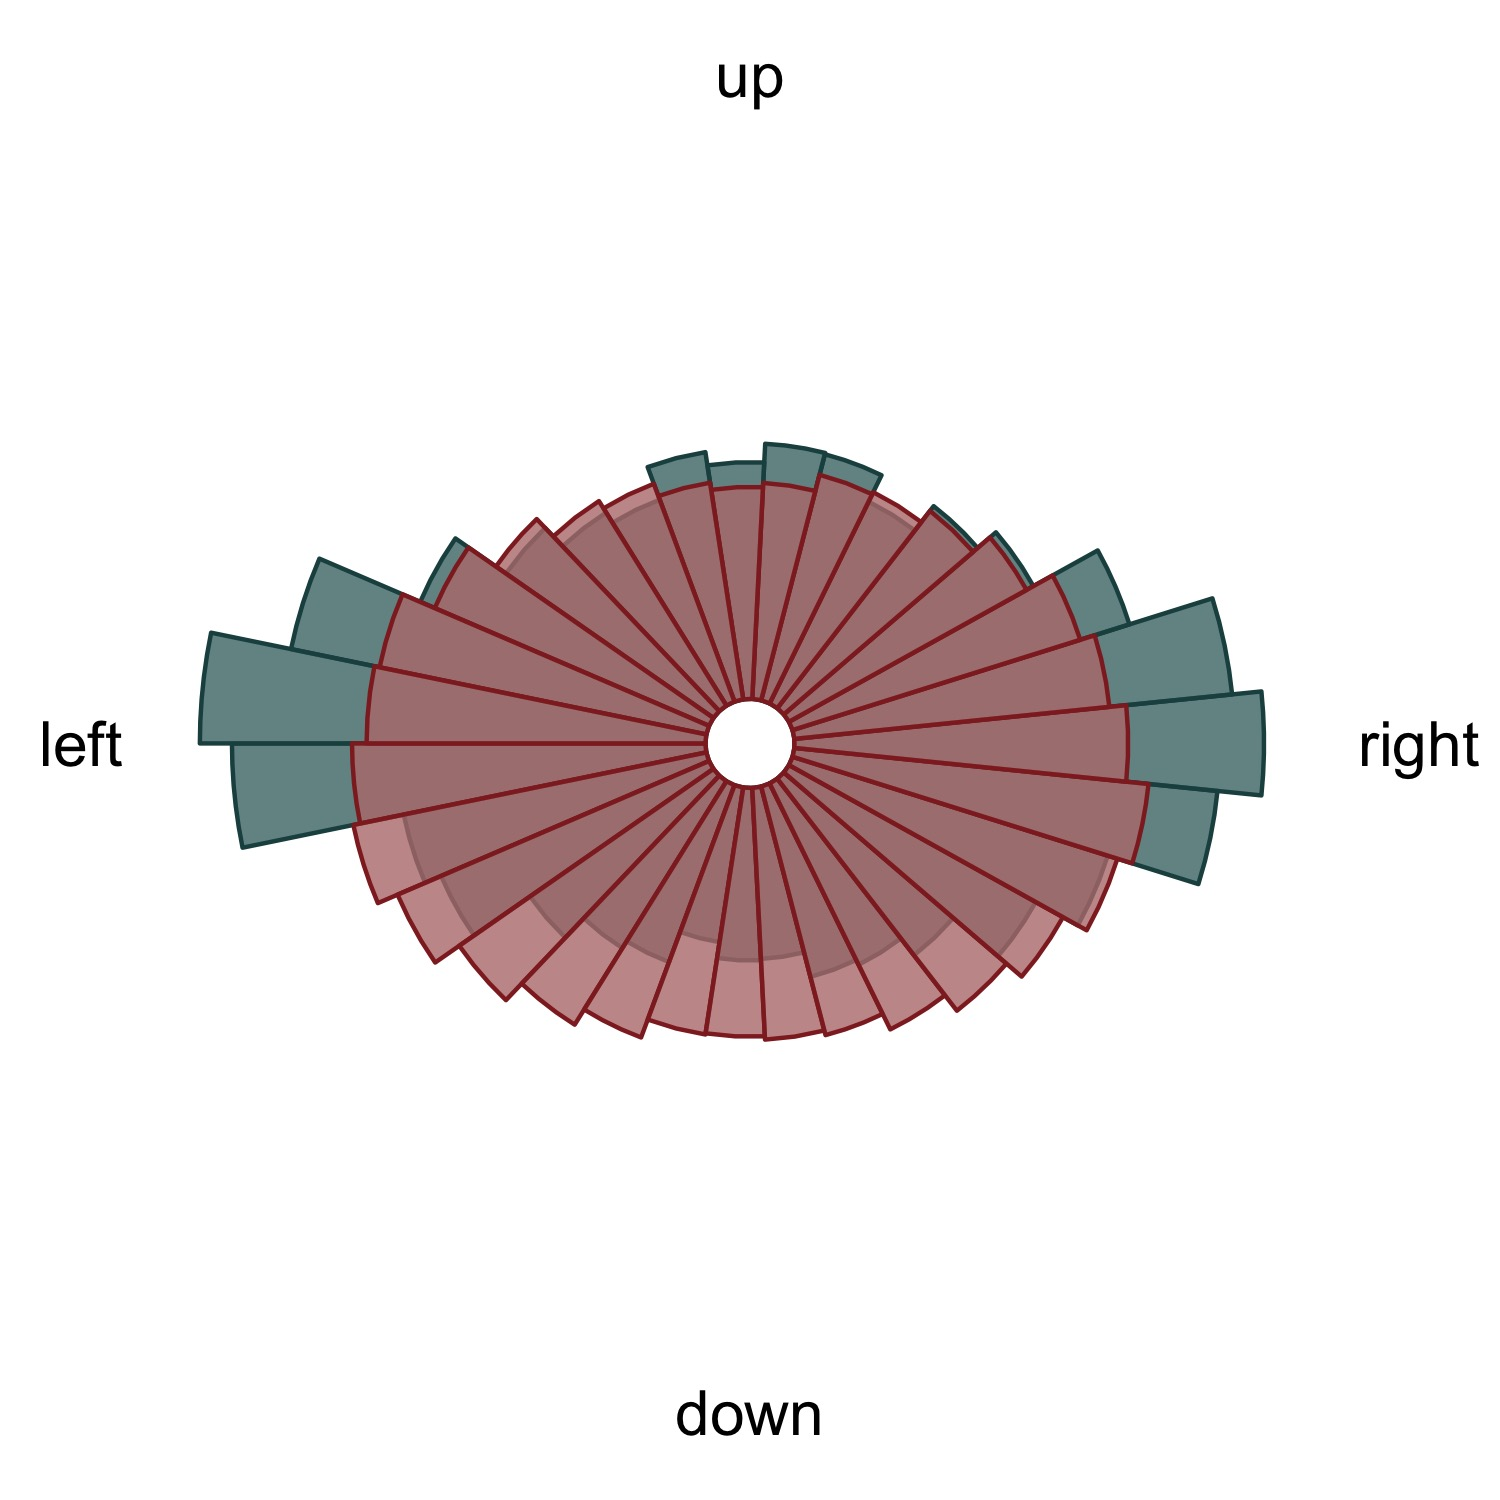
\includegraphics[width=0.45\linewidth]{figures/fit_model/in_sample/angle.jpg}
    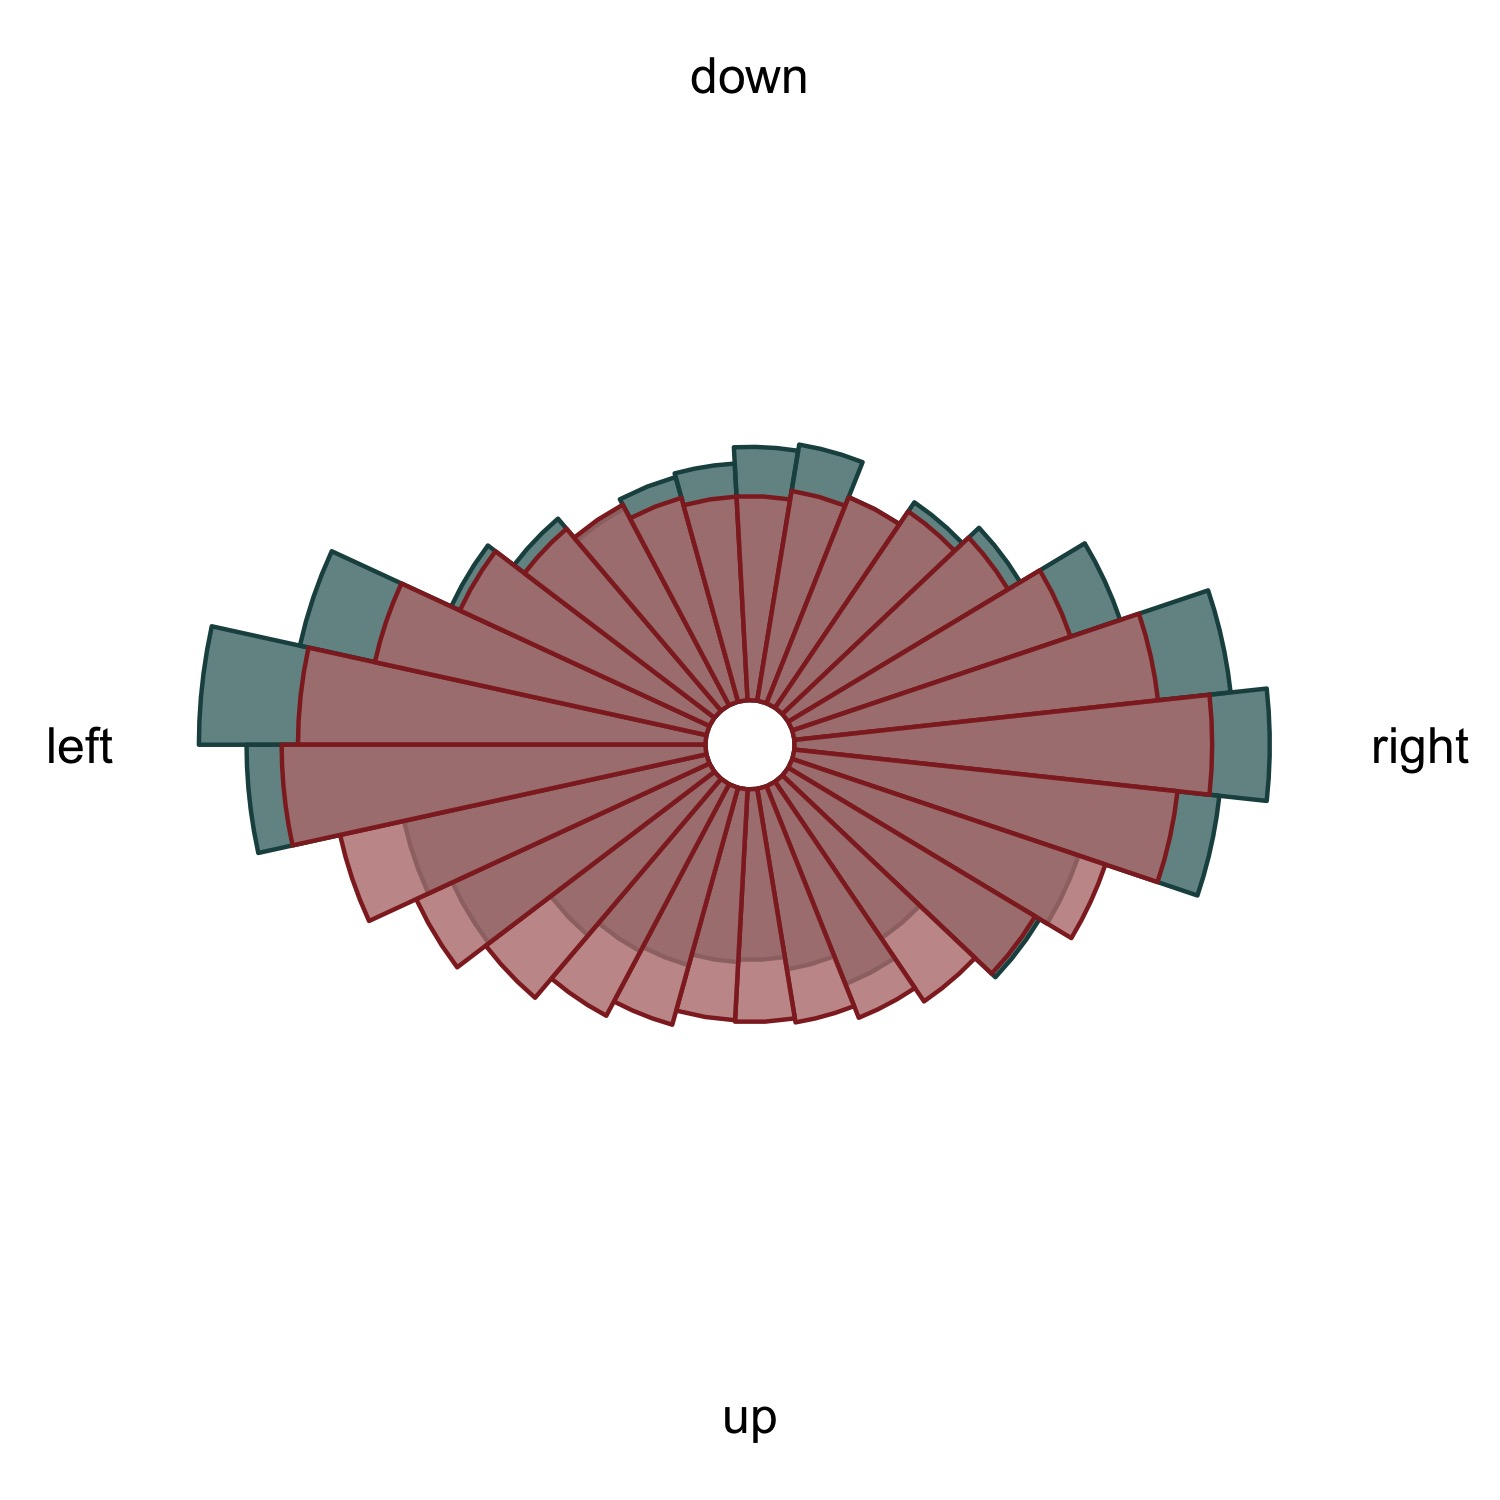
\includegraphics[width=0.45\linewidth]{figures/fit_model_horizontal/in_sample/angle.jpg}
    \caption{Predicted versus observed distribution of saccade angles under the initial (left) and extended (right) model, over all stimuli in the data set.}
    \label{fig:horizontal_comparison}
\end{figure}


\textit{Model comparison.} To assess whether the extended model did better at predicting the data compared to the initial model, we computed the log-likelihood of the hold-out set under the two models, given the posterior distributions of the parameters. This way, we obtained a distributions of the log-likelihood for the two models. To compare the two distributions, we computed the distribution of the log-likelihood differences: $\Delta \log \mathcal{L} = \log \mathcal{L}(\text{Model 2}) - \log \mathcal{L}(\text{Model 1})$: Positive values mean that the extended model predicted the hold-out data better than the initial model, and negative values mean that the initial model predicted the hold-out data better than the initial model.

The log-likelihood difference distribution (median=$45.77$, IQR$[15.18, 77.06]$) indicated that the extended model was better at predicting the hold-out data than the intitial model: adding horizontal bias into the model increased the model's predictive success.

\textit{Parameter estimates.} The estimates indicated that the most important factor were the objects on the scene (weight = $0.35$, $95\%\text{CI}[0.33, 0.37]$, followed by exploitation (weight = $0.31$, $95\%\text{CI}[0.29, 0.32]$, saliency (weight = $0.14$, $95\%\text{CI}[0.13, 0.16]$, central bias (weight = $0.13$, $95\%\text{CI}[0.11, 0.15]$, and lastly the horizontal bias (weight = $0.07$, $95\%\text{CI}[0.06, 0.8]$).

The parameters that control the individual factors were very similar to those of the initial model. The parameter that controls sizes of objects indicated that people fixate relatively close to the centroids of the objects (scale = $0.23$, $95\%\text{CI}[0.22, 0.24]$). The exploitation region had a scale ($\sigma = 34.28$, $95\%\text{CI}[32.80, 35.78]$) of about a third of that of the central bias ($\sigma=98.68$, $95\%\text{CI}[93.42, 103.99]$). The additional parameter that controls the concentration of the horizontal bias was estimated to $\kappa = 18.36$, $95\%\text{CI}[13.4,24.11]$.


\section{Conclusion and discussion}

In this article, we developed a new model to analyse eye movement data by specifying a joint probability distribution of the fixation duration and fixation locations. To our knowledge, this is the first attempt to model fixation durations and fixation locations by defining a joint likelihood function of these two random variables. Using Bayesian inference, we were able to fit and extend the model such that the predicted patterns of the fixation durations and fixation locations align very closely with those of the observed data. Drawing upon the strengths of specifying models using likelihood functions \citep{schutt2017likelihood}, we demonstrated how to diagnose, improve, and compare models so that they capture phenomena of interest present in real data. An example application showed that adding horizontal bias to the model improved model's ability to capture the distribution of saccade angles.

The model provides a relatively straightforward interpretation of the model parameters, facilitating the inference to what extent various explanations of eye movement events play a role. In our application, the results suggested that the most important factor determining eye movement behavior are the locations of objects on a scene, immediately followed by the tendency to make repeated fixations in a location nearby the current fixation. Salience and central bias had lower importance, and horizontal bias the least, although all factors made a valuable/significant contribution to fitting the model.

Although the final model fits relatively well, there are plenty of ways to make it better in the future. For example, previous research suggested that the central bias is slightly more stretched in the horizontal compared to the vertical dimension \citep{tatler2007central,clarke2014deriving}. In our application, we hold the width of the central bias in two dimensions equal. This could have created a slight misfit of the central bias factor, and could also underestimate the model's ability to produce saccade angles in the horizontal direction. Further, we hold the widths of factors in the model wherever possible to make the simplest model we could apply do the data, and so this limitation can relate also to the exploitation factor and the attention window (both of which we assume is spherical). Luckily, this issue can be solved easily in case the data indicate to do so.

Potential model misspecification could also arise from modeling the horizontal bias. It has been shown that von Mises distribution is not necessarily optimal for describing the distribution of the saccade angles, due to the fact that the real distributions of saccade angles are typically more peaked than what von Mises distribution allows \citep{mulder2020mixtures}. We used the von Mises distribution because it is relatively well known and can be fitted easily in Stan, whereas alternative distributions --- such as the power Batchelet distribution as proposed by \citet{mulder2020mixtures} --- would make the implementation much more complicated. A second potential misspecification of the horizontal bias could be that the current implementation assumes that at any point in time, it is equally likely to make a saccade to the left direction as to right direction. However, this is likely not true, as intuitively we could think that having a saccade very close to a left border of the scene would lead to a rightward saccade with a very high probability \citep{clarke2017saccadic}. This assumption can then underestimate the weight of the horizontal bias contribution compared to the other factors. 

Additional model misspecifications could arise from modeling many parameters as fixed across participants and stimuli. In the current model, we only modelled the most obvious source of individual differences --- the width of the attention window and the decision boundary --- as random between participants. However, it is probable that to better account for the patterns in the data \citep[and to justify generalizibility to a population of observers and a population of stimuli; ][]{yarkoni2019generalizability}, we could need to model many of the currently fixed parameters as random. For example, it is desirable to assume that participants can differ in the weights of the different factors, or that the importance of different factors are different even in different stimuli. Being able to generalize beyond the current data set was however not the focus of this article. However, the model is relatively flexible and including parameters as random should be possible in future applications.


It is possible that the proposed mechanism underlying the model's architecture is too simplistic or wrong. For example, our assumption is that observers linger on a current fixation for the time it takes to decide to move to another location. It is possible that instead observers linger on a current location for the time they harvest information from that location, or a completely different mechanism whatsoever. We also currently assume that the time it takes to select a new fixation location and plan a saccade is zero, and that observers plan new target fixations only one step ahead (ignoring pre-planned saccades). We also assume that different factors combine in an additive manner, which may not be the case \citep{barthelme2013spatial}. We believe that such alternative conceptual ideas could be contrasted with the current model by developing new mathematical and statistical models that concretely implement these. Having specific models that are derived from concrete theoretical assumptions will hopefully facilitate our understanding of the real generative mechanisms \citep{borsboom2020theory,schutt2017likelihood} that are relevant in eye-movement research. 

The current model made several assumptions for the sake of tractability. However, so far the results we have seen do not suggest that the model is performing poorly, and so we have a reason to believe that these assumptions are not particularly problematic.

We believe that similar attempts to modelling eye movements can influence both experimental practice as well as the theoretical advancements in the eye-tracking research. We hope that the current model will eventually be superseded by a better model --- which would be a good sign of a healthy progress of our scientific understanding of visual perception. In the meantime, we hope that the proposed model will spark interest in applied and theoretical research of eye movements and provide valuable insights.

\bibliography{bibliography}

\end{document}
